\documentclass{ltjbook}
\usepackage{docmute} 
\usepackage{../../myStyle} 

\begin{document}
\VerbatimFootnotes
\chapter{Practical Bayesian Estimation with JASP}
\label{m28_jasp}
In the previous discussion, we introduced methods for using Bayesian estimation to make judgments, such as using HDI and ROPE, and using the Bayesian factor.

Let's learn specific methods for performing Bayesian estimation, as merely sketching out methods without being able to actually compute them would be like drawing pictures of mochi.
\section{Methods for Bayesian estimation}
\subsection{Analytical Methods}
To actually perform Bayesian estimation, it is well understood that one can simply use the Bayes' theorem to make the calculation.
Bayes' theorem was as follows:
\[ P(A|B) = \frac{P(B|A)P(A)}{P(B)} \]
You are right, indeed we can calculate it this way. However, for instance, if we want to use this calculation method to find the mean $\mu$ and standard deviation $\sigma$ of a normal distribution, the $P(B|A)$ is the likelihood function.
\[ P(X|\mu,\sigma) = \prod_{i=1}^N \frac{1}{\sqrt{2\pi \sigma}}exp\left( - \frac{(X_i-\mu)^2}{2\sigma^2}\right) \]
This can be expressed as follows. Next, the prior distribution, $P(A)$, represents the prior belief about the parameters, so we need to represent $P(\mu,\sigma)$ as some probability distribution. As it is a multidimensional probability distribution, we can sense that it could become complicated.
The denominator $P(B)$ is the marginal likelihood of the model over the entire parameter space, given by the calculation $\int_\mu \int_\sigma P(X|\mu,\sigma)P(\mu,\sigma) d\mu d\sigma$. The symbol $\int \int$ represents the integration, but the calculation becomes quite complex due to multiple integrations. In this case, there were two parameters, but when there are more, the calculation becomes practically impossible. While Bayes' theorem itself has been known for a long time, one reason why it was not put into practical use is because of the complexity of this integration calculation.

If you still want to perform Bayesian estimation, the way to do it is to find a "prior distribution that has the same functional form as the posterior distribution." For example, if the likelihood is the Bernoulli distribution or the binomial distribution, assuming a beta distribution as the prior distribution results in a posterior distribution with the same beta distribution form. This becomes apparent by expanding the calculation formula, and such distributions that have this property are referred to as conjugate prior distributions. Occasionally, these special combinations can be found, and if successful, the answer can be obtained through calculation. However, if the parameters become more numerous, the posterior distribution becomes a shape that is difficult to understand, a form that cannot be calculated even though the formula can be written, or something that cannot be generalized, and it becomes impossible to proceed.
\subsection{Grid Search}
The next method to be introduced is called grid search. In Lecture \ref{m26_bayesian2}, we used the following expression:
The formula translates to: "The posterior distribution is proportional to the likelihood multiplied by the prior distribution, without modifying the TeX code."
This means that when computing the posterior distribution, it is sufficient to focus on the proportional relationship $\propto$ and ignore the denominator. This is because the denominator is just a number used to ensure that the area under the curve is 1, i.e. to convert the product of the likelihood and prior distribution into a probability. What we are interested in is the peak of the posterior distribution, such as the MAP estimate, and the shape and slope of the distribution. Hence, as long as we know the shape and slope of the distribution, we do not need to worry about the actual values of the posterior distribution.

So, let's express the prior and posterior distributions as a formula without modifying the TeX code (this is tedious, but it can be done if you try). For example, if we have a combination of the Bernoulli likelihood function and the Beta distribution, the parameter is only $\theta$, so we divide the parameter into appropriate sizes and substitute them into the formula to find where the probability becomes high. If it seems like the peak of the posterior distribution is higher for $\theta=0.6$ than for $\theta=0.3, we can further divide the parameter into smaller sizes like $\theta=0.55,0.575,0.600,0.625$...and repeat the process to get an approximate estimation of "the peak is around here." Computers are good at this kind of iteration, so it should be possible with enough time. By the way, of course, this is just an example chosen to simplify the explanation, and in reality, it becomes a story about applying it to more complex models. For a normal distribution model, the two parameters, $\mu$ and $\sigma$, are divided into smaller sizes. The divided sections are called grids, so searching by dividing into grids is called grid search.

While this method may be effective in finding peaks, there is the possibility of missing out on even higher peaks if the posterior distribution has multiple peaks like a mountain range. Additionally, as the number of parameters increases, the computation becomes much more time-consuming, rendering this method impractical as a solution. It is safe to say that this approach is not a realistic solution to the problem.
\begin{figure}[ht]
   \centering
   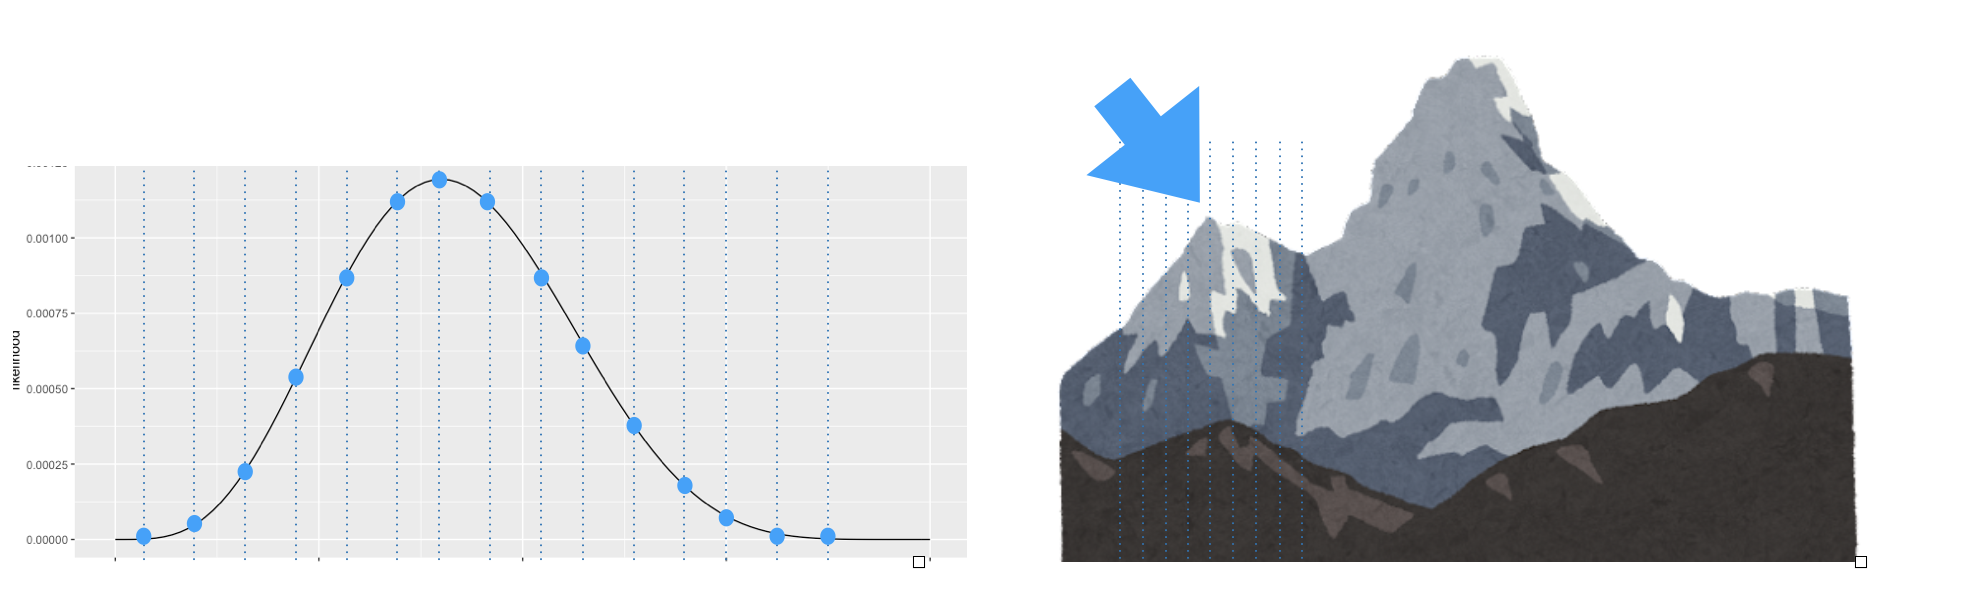
\includegraphics[keepaspectratio,width=0.8\linewidth]{../images/28_JASP/slide28_01.png}
   \caption{Grid search method for finding peaks by slicing}
   \label{fig::28_01}
\end{figure}

\subsection{Markov Chain Monte Carlo Method}
Finally, we must mention the significant contributions that Markov Chain Monte Carlo (MCMC) methods have made to the advancement of modern Bayesian statistics.
This method, known as MCMC (Markov Chain Monte Carlo), combines two techniques: Markov chains and Monte Carlo algorithms. A Markov chain, also known as a Markov process, is a method of creating transition rules that will lead to the desired probability distribution state. Monte Carlo methods, on the other hand, are algorithms that generate random numbers. By combining these two techniques, it is possible to create a random number generator that can provide samples even when the shape of the probability distribution is unknown.

As mentioned briefly in Section \ref{randomVariablesMethod} on page \pageref{randomVariablesMethod} of Lecture \ref{m07_probability}, one approach to approximating probability distributions is by generating random numbers. In R, common probability distribution functions such as the normal distribution, binomial distribution, t-distribution, and F-distribution are preloaded and ready to use. For example, by using \verb|dnorm|, one can calculate the density of the normal distribution (\verb|norm|), and by using \verb|qt|, one can get the probability point (\verb|q|) of a certain range in the t-distribution. Additionally, the function \verb|rnorm(N,mean,sd)| can generate N random numbers with any mean and standard deviation. By generating a large number of random numbers, the resulting histogram reproduces the shape of the normal distribution as shown in Figure \ref{fig::28_02}.
\begin{figure}[ht]
	\centering
	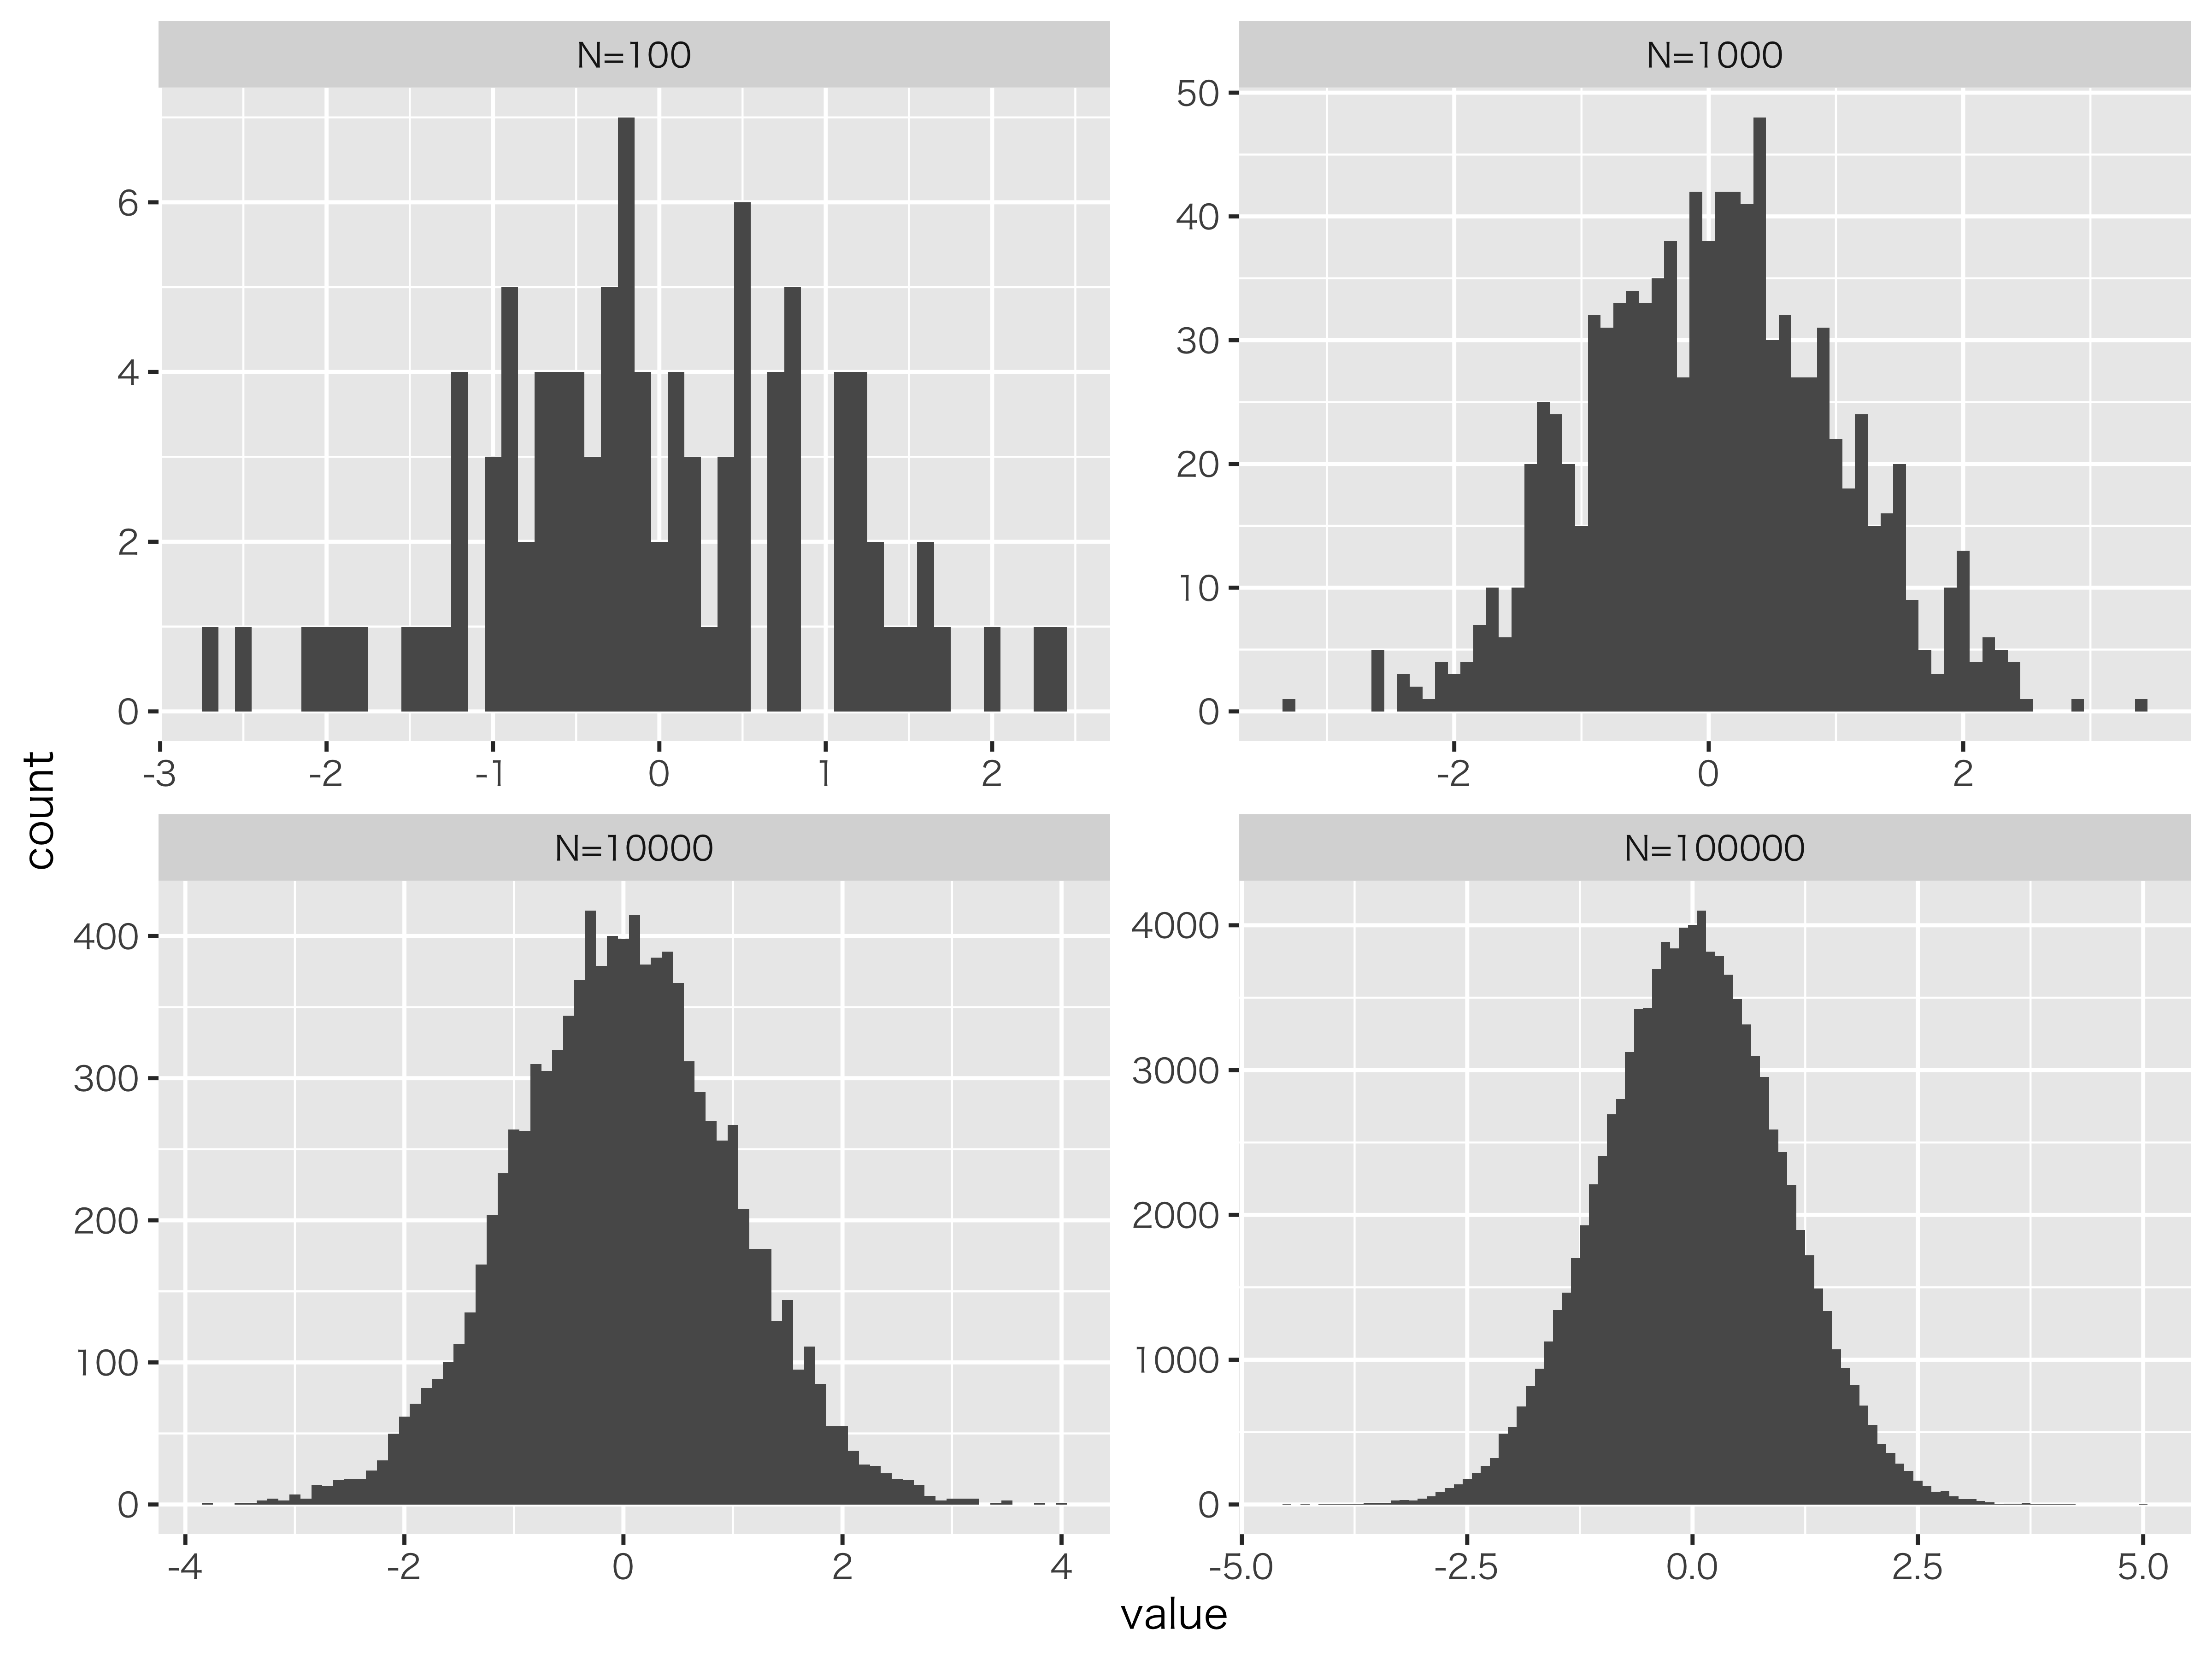
\includegraphics[keepaspectratio,width=0.65\linewidth]{../images/07_probability/Rplot08_06.png}
	\caption{As the number of random numbers increases, the shape of the normal distribution approaches. Histograms plotted by generating 100, 1000, 10000, and 100000 points of random numbers from the top left.}
	\label{fig::28_02}
\end{figure}


Generating random numbers within a computer is purely \textbf{pseudo}. This is because the world inside the computer is a fully calculated world. It is contradictory to generate "regular" and "irregular" number sequences. In computer science, various studies have been conducted on how to generate numbers that follow a calculation rule, but appear random. One of these random number generation techniques is the \textbf{Monte Carlo method}\footnote{By the way, Monte Carlo is a city in Monaco where casinos are famous. This name is given because it generates random numbers like a roulette at a casino.}.

However, what we are interested in is the posterior distribution. If we could approximate the posterior distribution with random numbers, it would be beneficial. However, the form of the posterior distribution is an unnamed probability distribution that cannot be generalized, even though it can be expressed mathematically. There is a method called \textbf{Markov chain} to connect the state of the posterior distribution to the technique of generating random numbers. Markov chains are models of probability transition states that study stabilizing the transition patterns in a situation where the state of time t is determined by the previous step, t-1. By adjusting this stabilized pattern to become the posterior distribution and generating random numbers for each transition step, a sequence of representative numbers for the posterior distribution can be obtained.

In essence, a method has been developed to generate random numbers from \underline{any probability distribution}, without changing the TeX code. While the function of the posterior distribution may be complex, generating a large number of random numbers from it allows us to draw a histogram that represents the shape of the posterior distribution. With modern statistical environments, it is easy to compute large amounts of data and create corresponding visualizations. Data processing for tens or hundreds of thousands of data points (MCMC samples from the posterior distribution) can be accomplished in just a few moments.

One advantage of this random number generation method is that it is not difficult to deal with multiple parameters. When you have two parameters, $\mu$ and $\sigma$, that you want to find, the parameter values are spread out in a two-dimensional space. For example, if you want to know the distribution of only $\mu$, you have to analytically integrate $\sigma$ over the entire range and eliminate it \footnote{This is the process called \keytermE{marginalization} that we did in the previous session.}.

However, when it comes to random number generation, there is no particular need to be conscious of integration or marginalization elimination. Figure \ref{fig::28_03} shows a scatter plot generated from random numbers in two-dimensional space, as well as the corresponding density plot after marginalization. This density plot essentially just shows a histogram of each variable. By considering each variable individually, one can effectively eliminate the influence of other variables, without needing to consider cumbersome calculations such as integration.
\begin{figure}[ht]
	\centering
	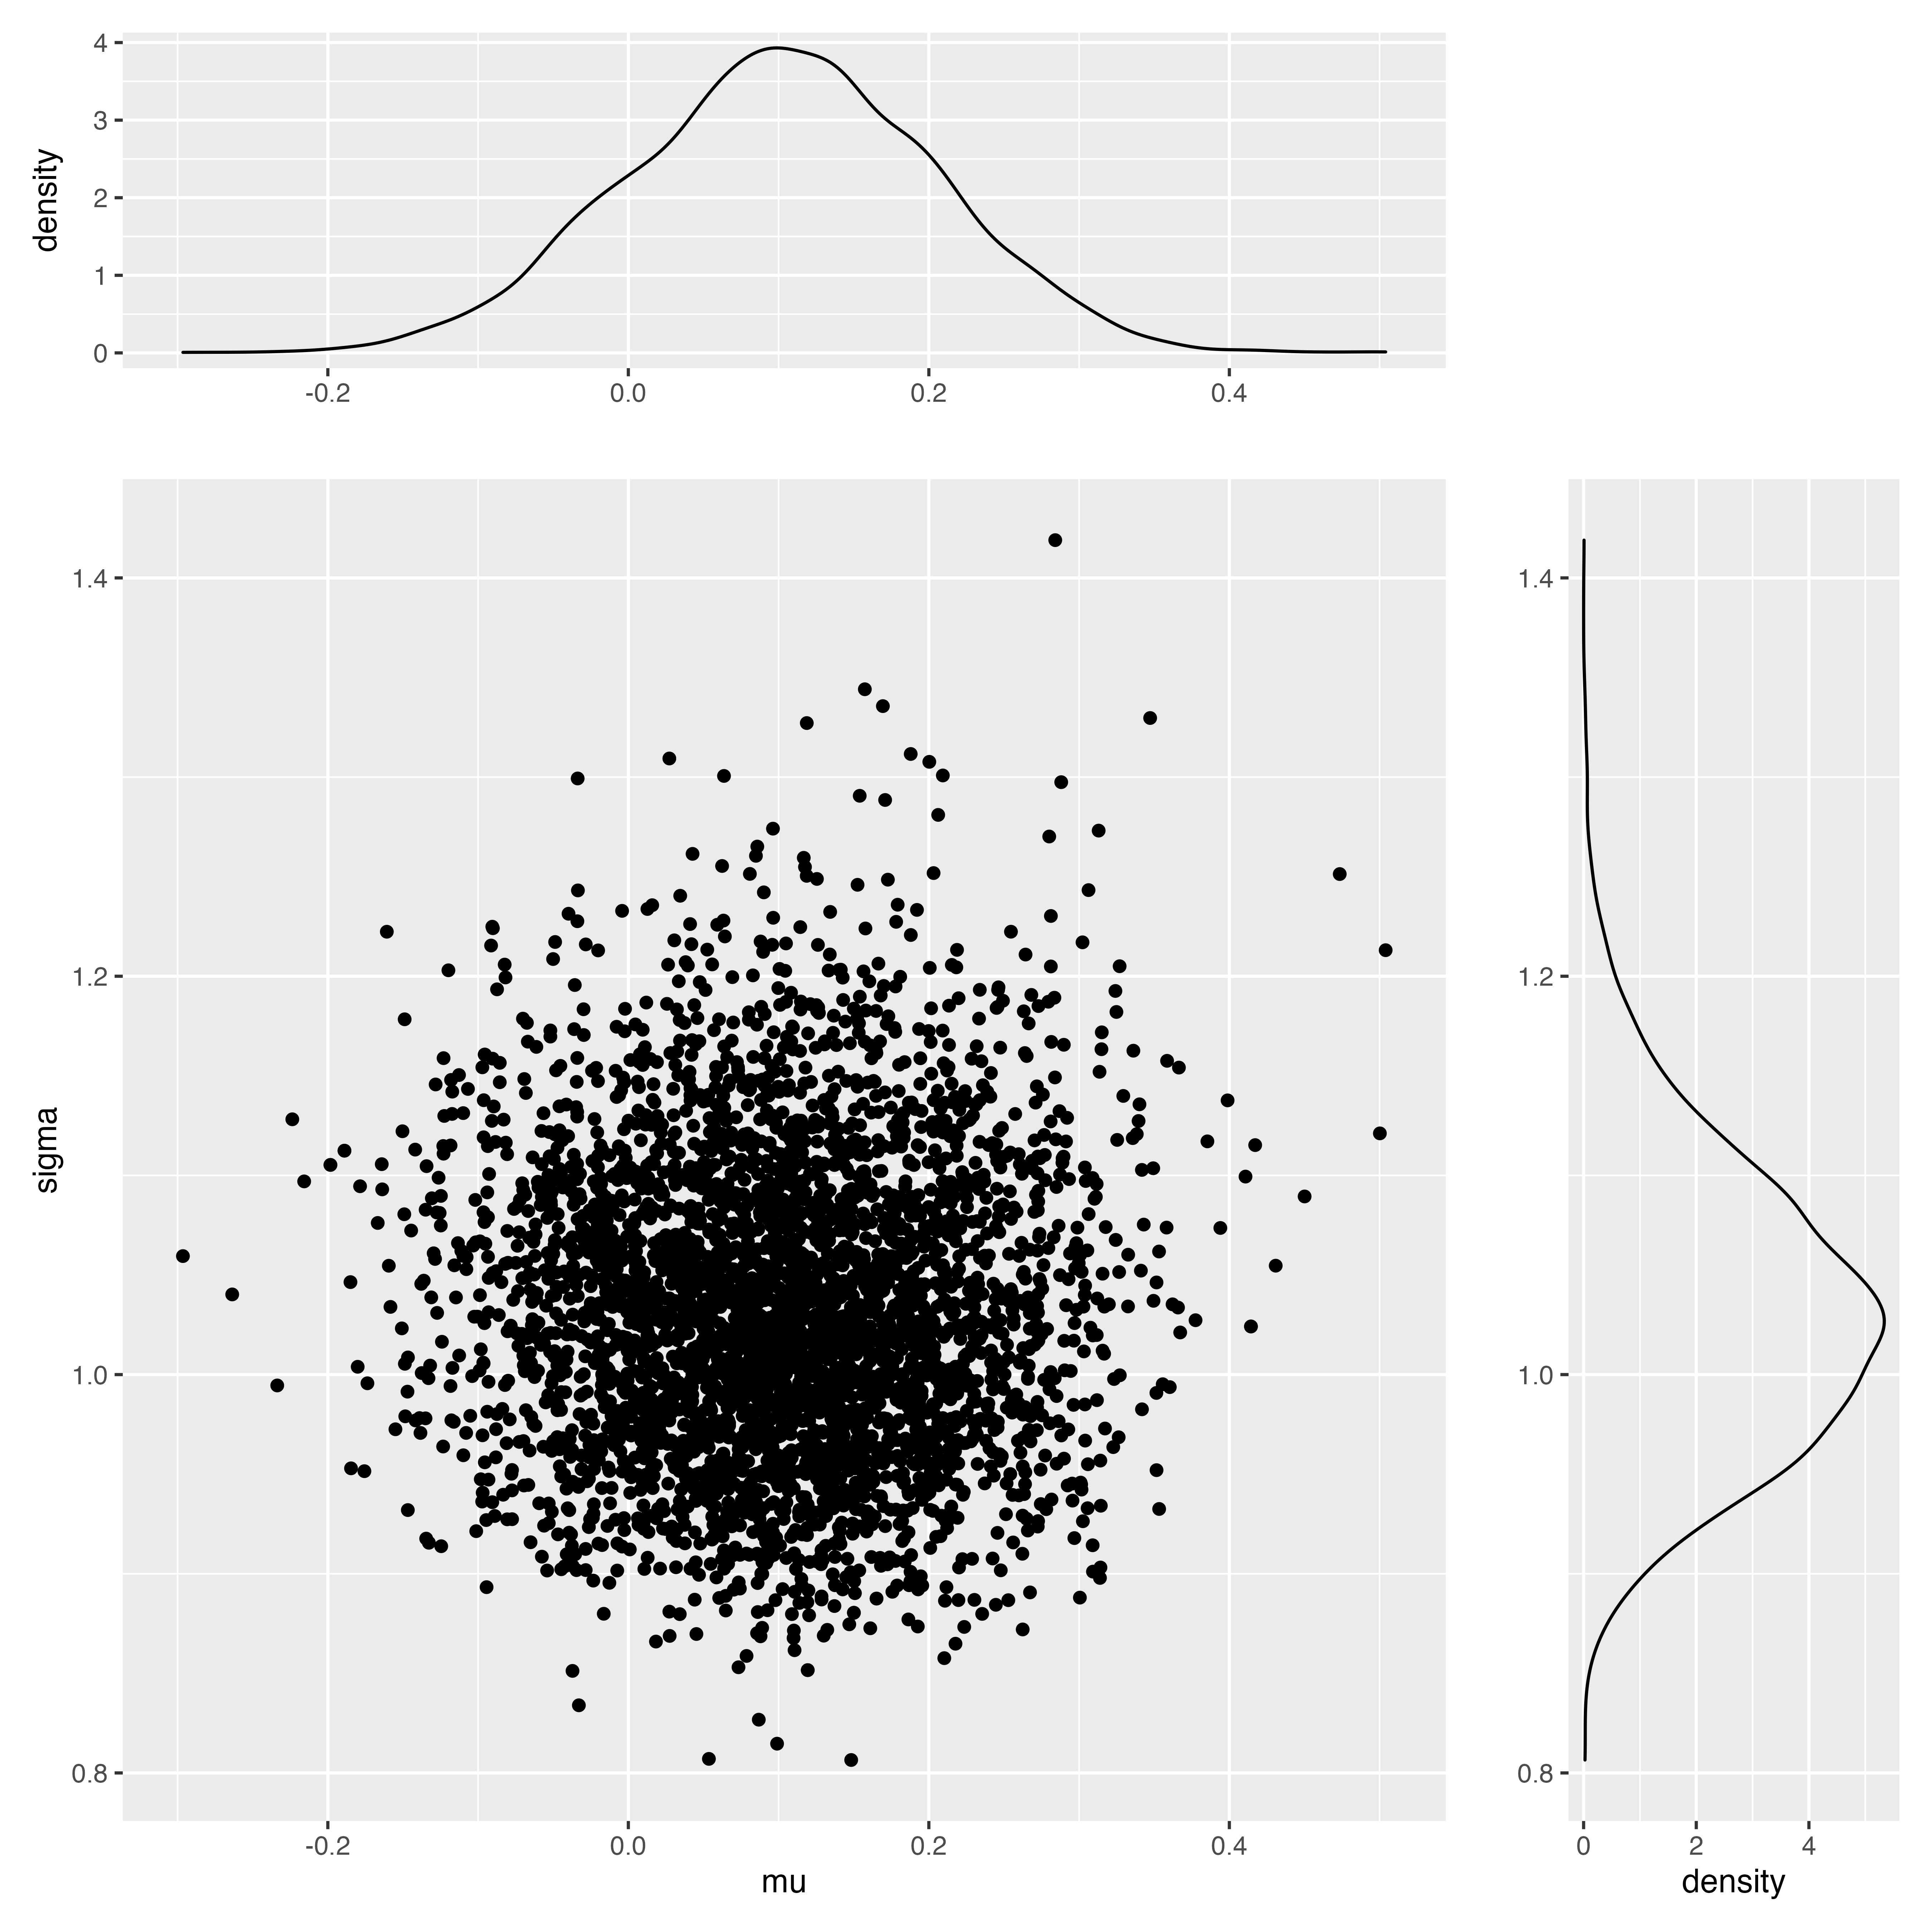
\includegraphics[keepaspectratio,width=0.65\linewidth]{../images/28_JASP/Rplot28_01.png}
	\caption{Marginalization is achieved through histograms of individual variables}
	\label{fig::28_03}
\end{figure}


Using random numbers, integration calculations become easy. Even in multi-dimensional cases, you only need to aggregate the variables of interest, and partial aggregation of a variable (parameter) becomes the integration over that range. There is no easier or more reliable way than this.

Thanks to the use of these MCMC methods, it has become easy to practice Bayesian statistics. To implement this MCMC method, a programming environment with a random number generation function is required. Several representative languages, called stochastic programming languages, can be used for this purpose, such as JAGS \citep{JAGS} and Stan \citep{stan2017}. These languages can calculate the product of likelihood and prior distribution by setting data, probability models, and prior distributions, and then generate random numbers from the result. These languages must be used in conjunction with other statistical environments such as R. R can use packages such as rstan and cmdstanr to communicate with Stan, and perform aggregation and visualization. (See Figure \ref{fig::28_04}).
\begin{figure}[ht]
   \centering
   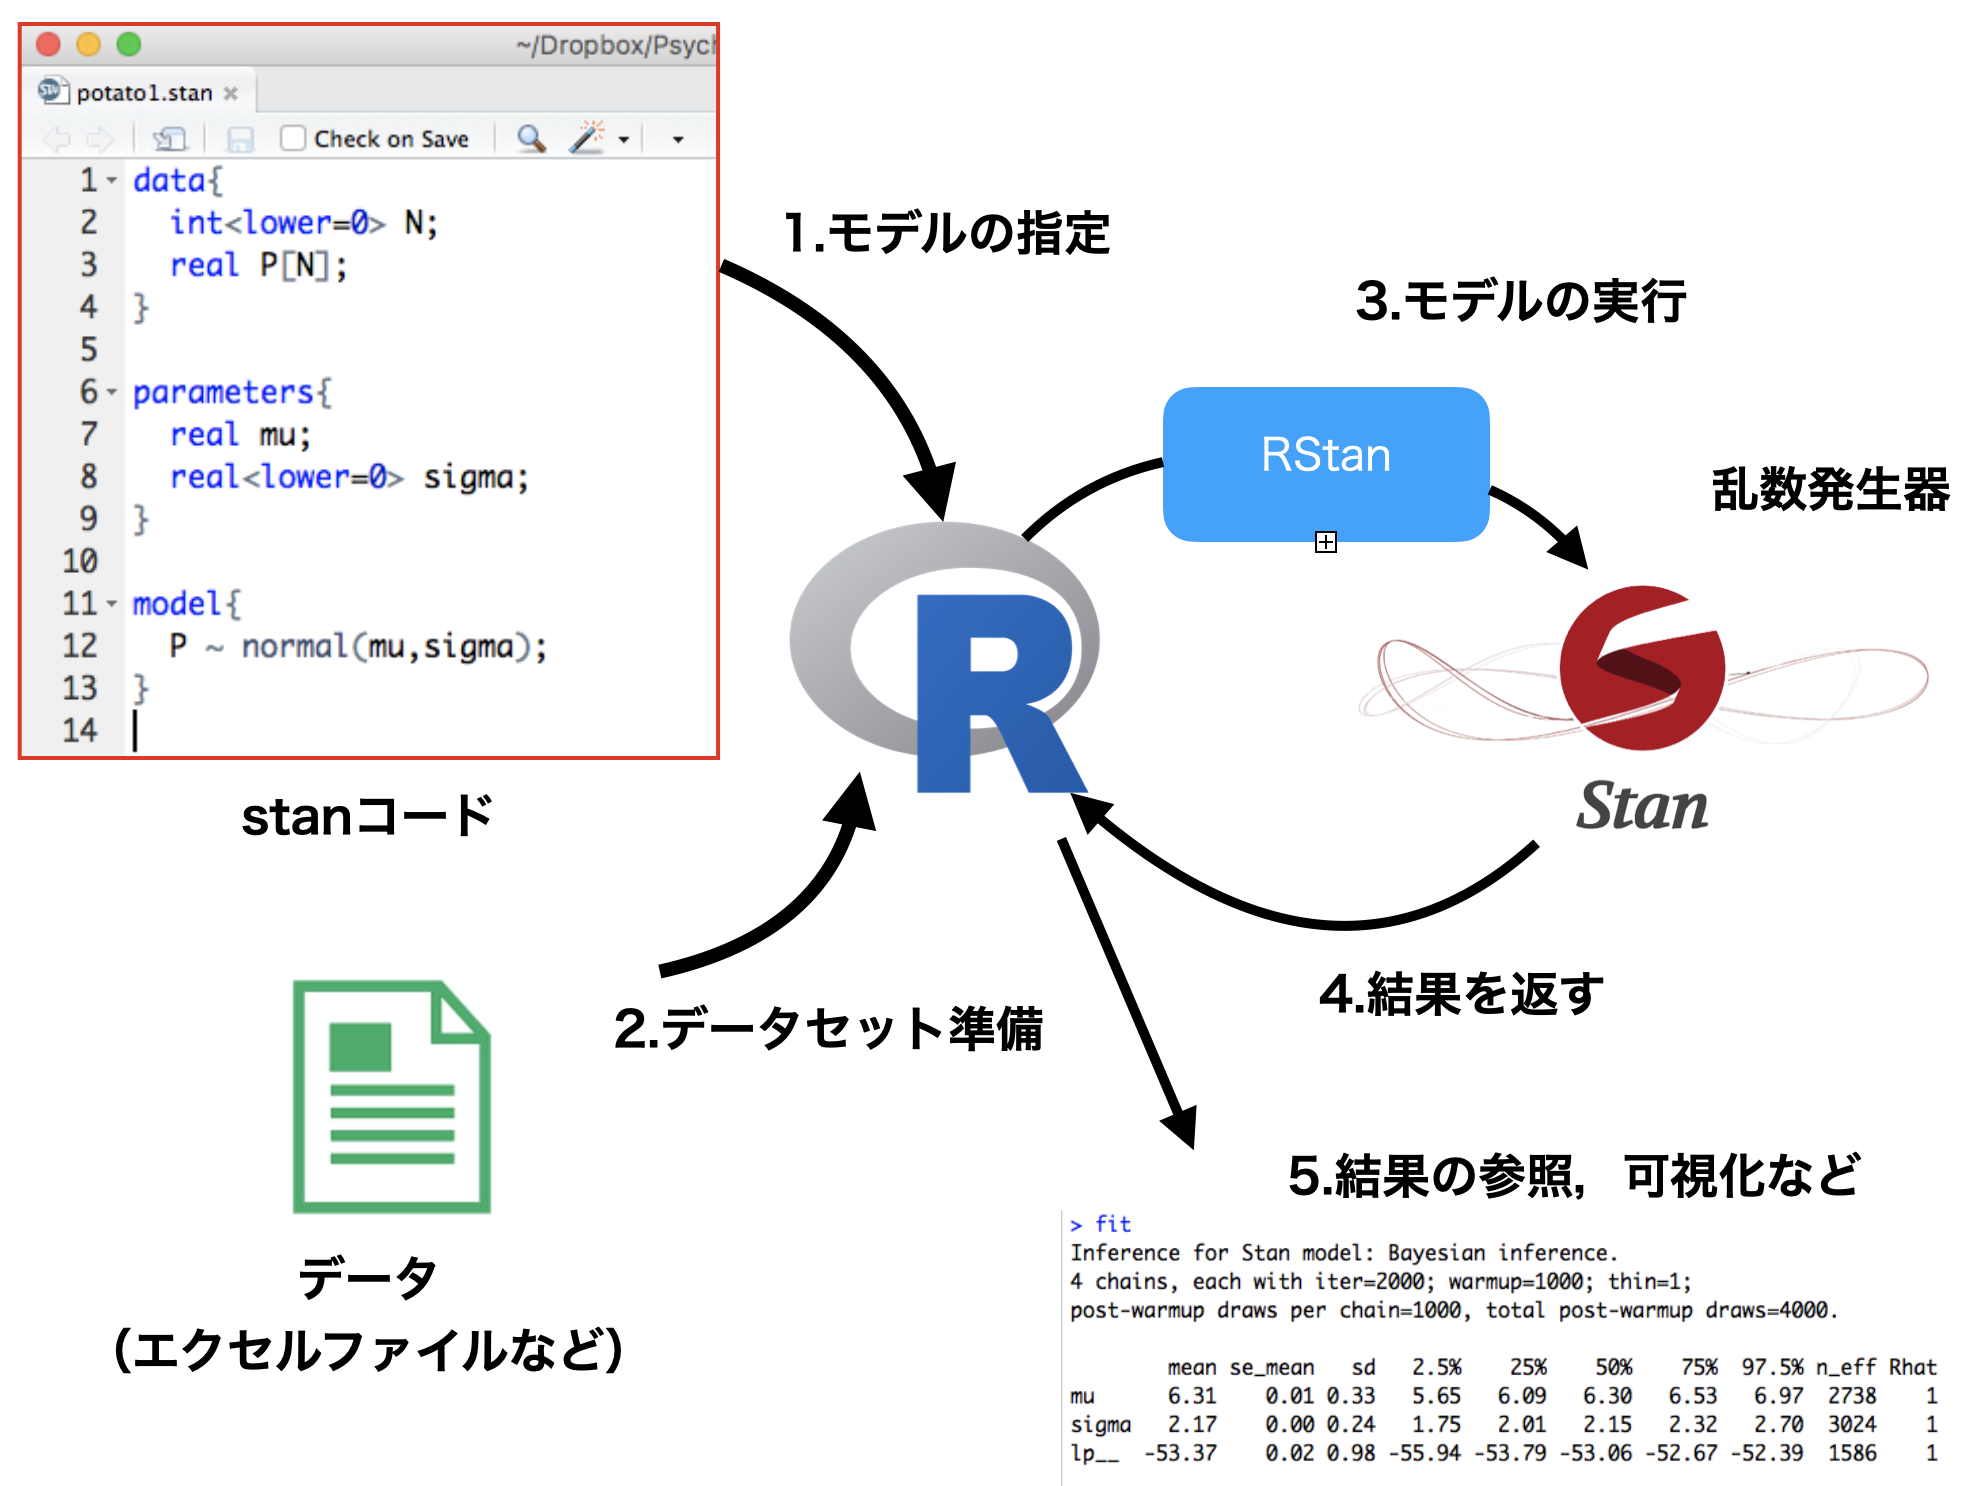
\includegraphics[keepaspectratio,width=0.65\linewidth]{../images/28_JASP/slide28_02.png}
   \caption{Image of using Stan from R}
   \label{fig::28_04}
\end{figure}


The program code for Stan, including the recipe for generating random numbers, can be edited on RStudio, allowing for Bayesian analysis to be conducted.

Some people may feel that it is still difficult and daunting. But don't worry, there are R packages available, such as "brms" \citep{brmsCite1,brmsCite2} and "blavaaan" \citep{blavaanCite1,blavaanCite2}, that allow you to use Stan for analysis without writing Stan code.
There are also statistical packages that make Bayesian analysis much easier, without modifying the TeX code. Let's take a look at one such incredibly simple statistical analysis software called \keytermE{JASP}{JASP}.

\section{Introduction to JASP}
JASP is also a free software, like R. This is an open-source project supported by the University of Amsterdam.
If you search for JASP, you'll be directed to the main site \url{https://jasp-stats.org/} (see Figure \ref{fig::28_05}). At the time of writing this text\footnote{December 17th, 2021 at 2:48 pm}, the latest version is ver0.16.
\begin{figure}[ht]
	\centering
	
\includegraphics[keepaspectratio,width=0.65\linewidth]{../images/28_JASP/JASP_web01.png}
	\caption{JASP website}
	\label{fig::28_05}
\end{figure}

Here, there is a download button (Download JASP) which, when clicked, provides access to JASP compatible with various operating systems.
Download the version that suits your environment, and try installing the app\footnote{macOS users who manage software packages using Homebrew can install it with \verb|brew install JASP --cask|.}.
\begin{figure}[ht]
   \centering
   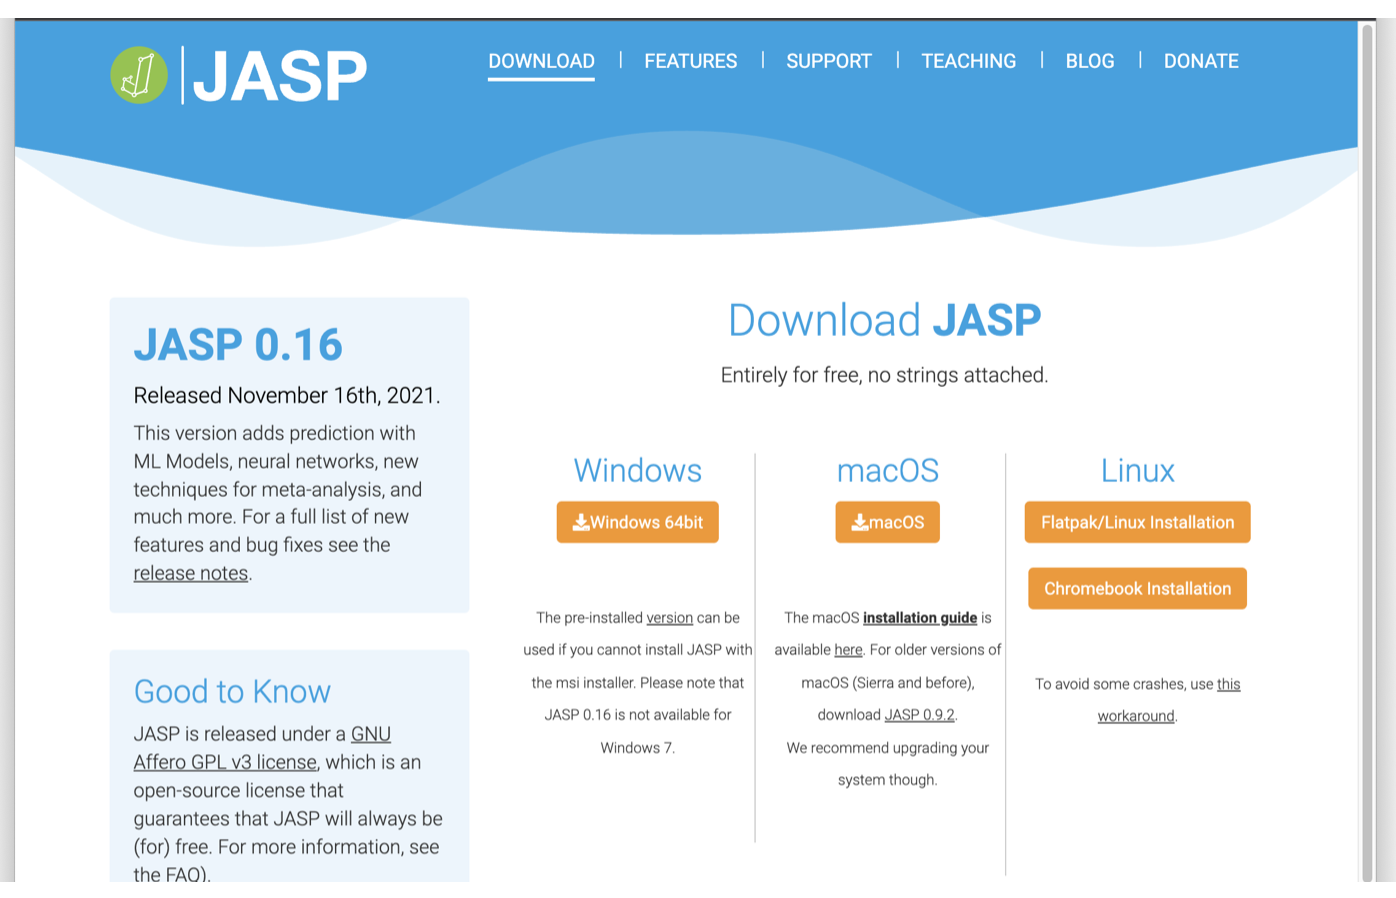
\includegraphics[keepaspectratio,width=0.65\linewidth]{../images/28_JASP/JASP_web02.png}
   \caption{Download the version that suits your environment}
   \label{fig::28_06}
\end{figure}

Once the installation process is completed successfully, let's try to launch JASP. I believe that the startup screen for JASP has already been translated to Japanese. There, you will find an explanation of JASP's characteristics which include \textbf{Free, Friendly, and Flexible}. In particular, the description of "Flexible" emphasizes that this software seamlessly combines traditional and Bayesian analysis methods, which is a unique feature not found in any other package.
\begin{figure}[ht]
   \centering
   
\includegraphics[keepaspectratio,width=0.65\linewidth]{../images/28_JASP/JASP_wakeup.png}
   \caption{Please also read the greeting on the startup screen.}
   \label{fig::28_07}
\end{figure}


There is also a statement below that says, "JASP is being developed at a furious pace!" Although the version of JASP is not yet even 1.0, it has already reached a level of usability and development is continuing. By the way, the author is also part of the Japanese localization team\footnote{For more details, see \url{https://jasp-stats.org/2021/10/28/日本語でjaspが使えるようになりました/}}, so if there are any unnatural translated terms, misspelled words, or mistranslations, please let us know\footnote{Or you can contact the JASP users' group at \url{https://github.com/jasp-user-jp/jasp-user-jp}.}.

Let's try it out a little bit.
Click on the three lines in the top left corner of the screen to open the main menu. From here, select "Open" -> "Computer" to load data files from your own PC.
\begin{figure}[ht]
	\centering
	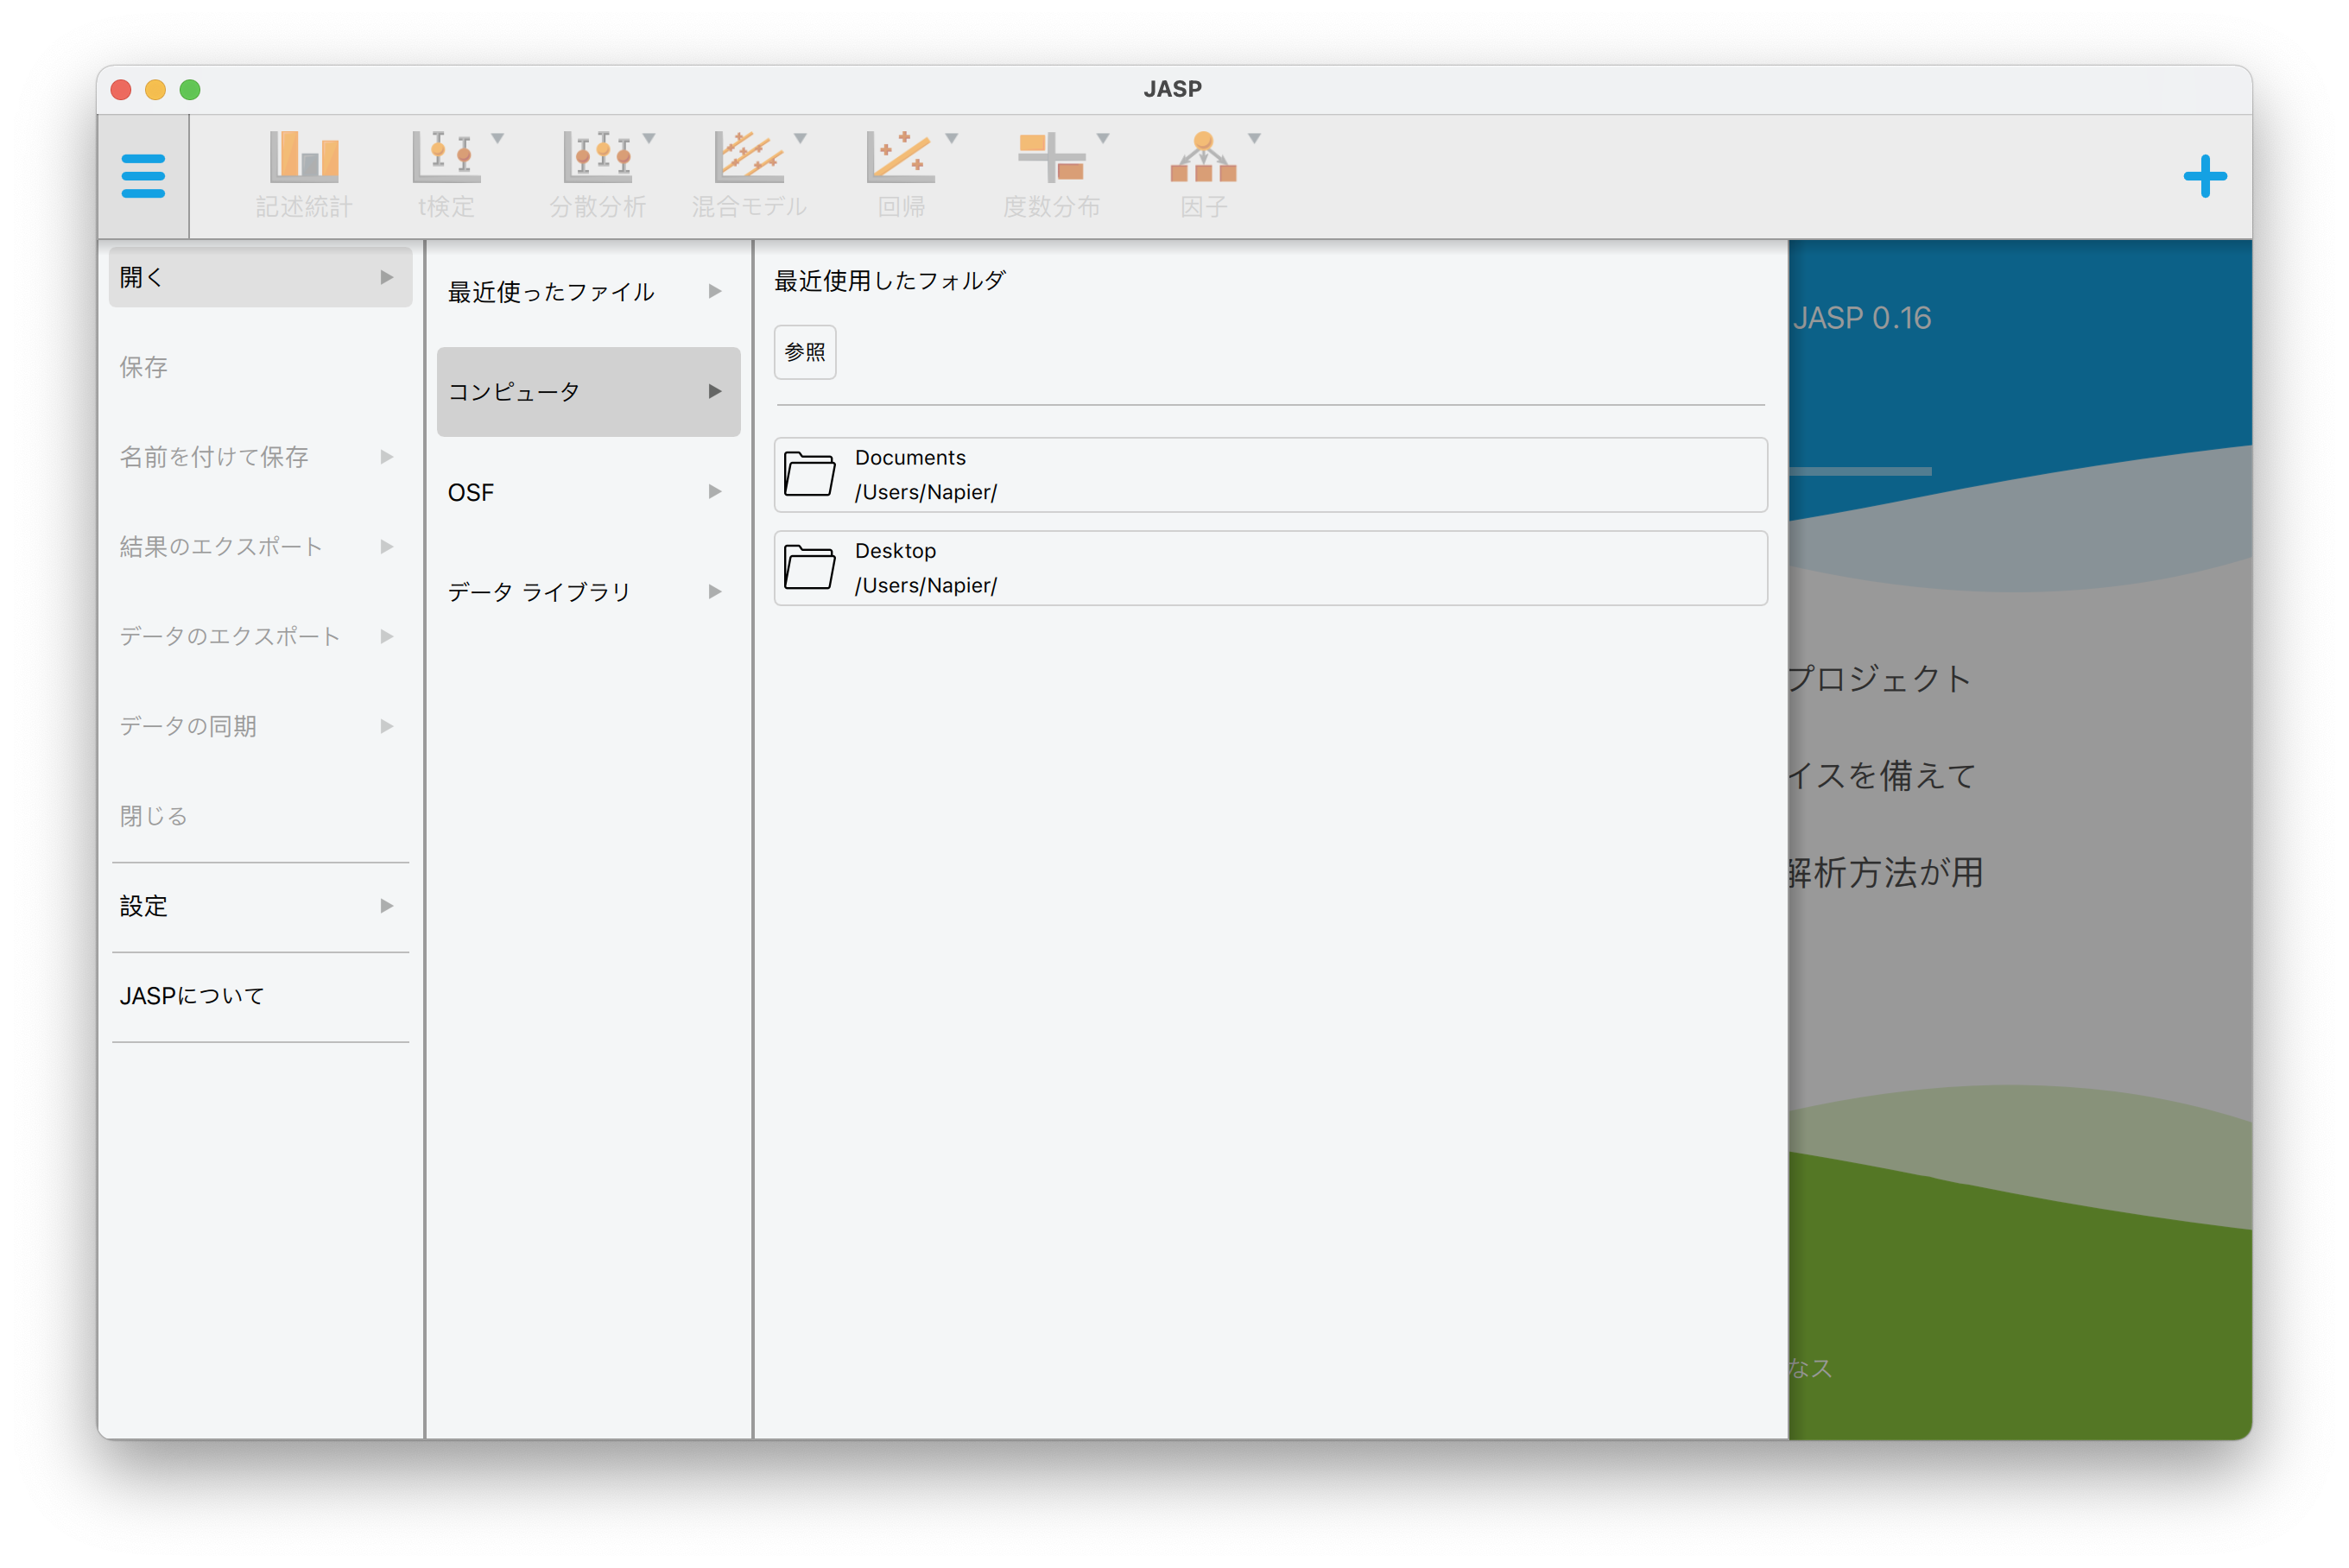
\includegraphics[keepaspectratio,width=0.75\linewidth]{../images/28_JASP/JASP_01.png}
	\caption{Read file}
	\label{fig::28_08}
\end{figure}

As an example, let's try to read a data file (csv) of baseball players.\footnote{This sample data is provided on the accompanying website of this article.}
\begin{figure}[ht]
   \centering
   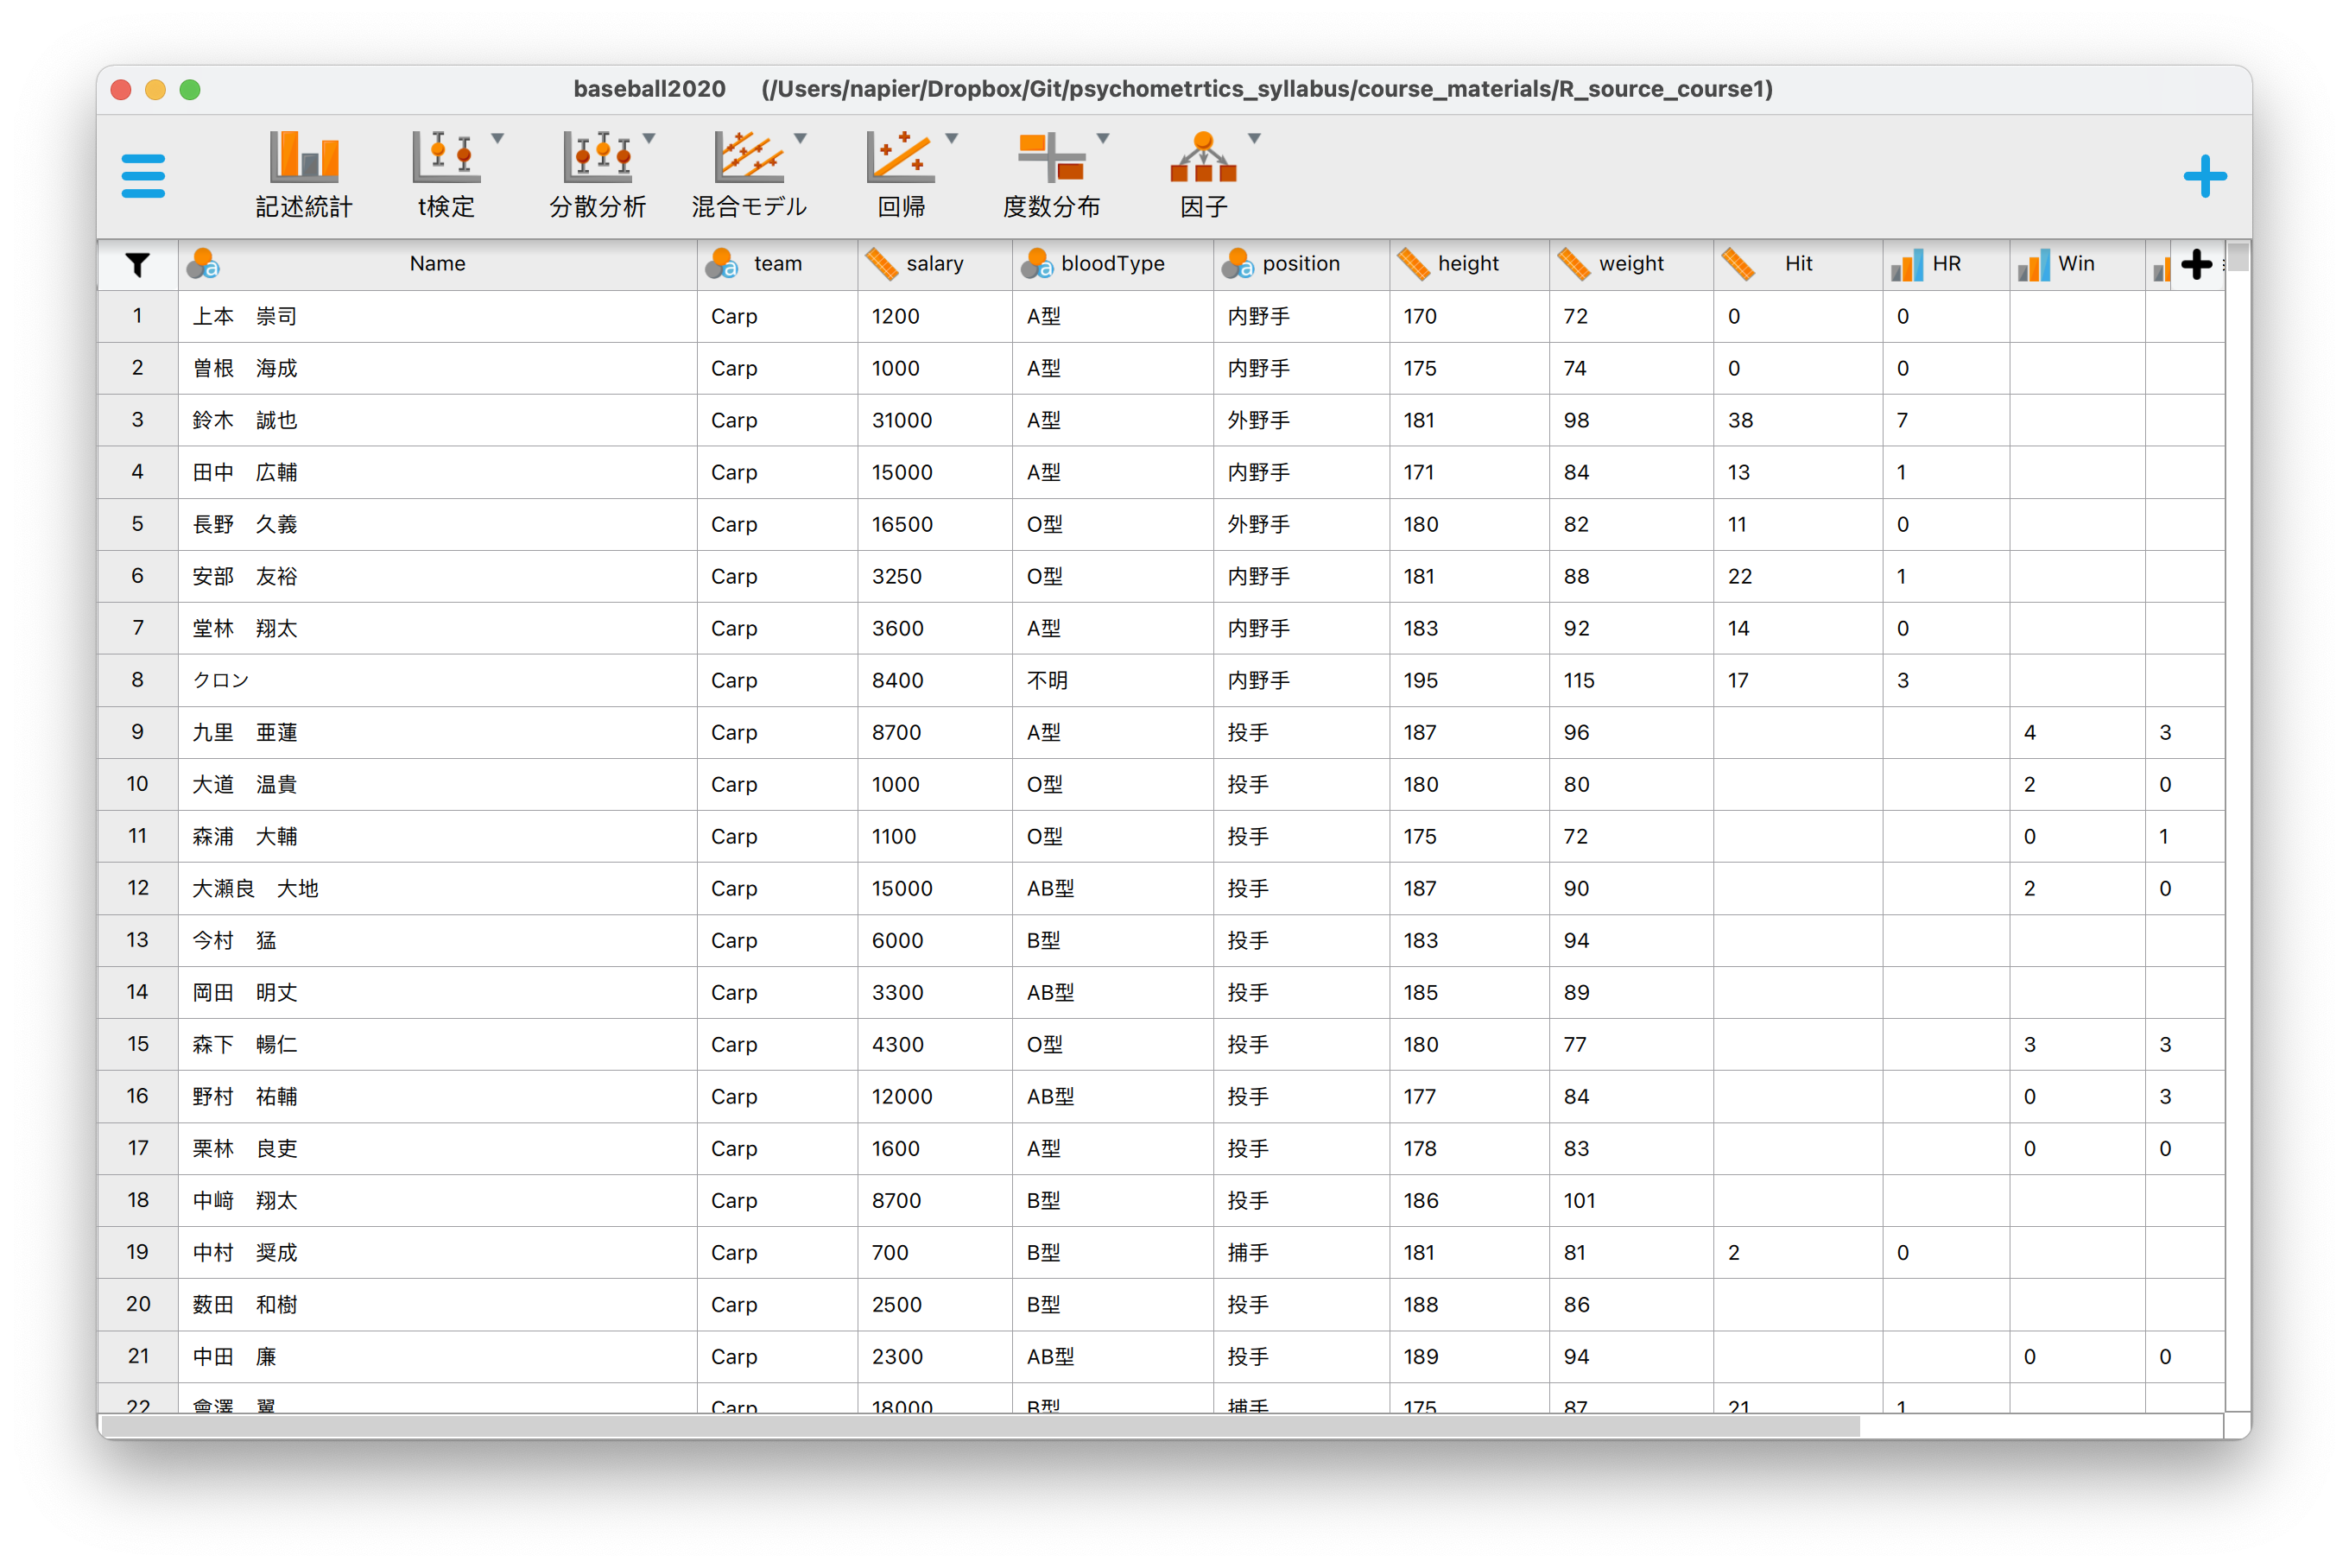
\includegraphics[keepaspectratio,width=0.75\linewidth]{../images/28_JASP/JASP_02.png}
   \caption{File loaded successfully}
   \label{fig::28_09}
\end{figure}

Once loaded, the data file will be displayed. You may notice that some variables have symbols next to them, such as those resembling Venn diagrams or measuring scales. In JASP, data is classified into three types: \textbf{nominal}, \textbf{ordinal}, and \textbf{scale}. Scales are a combination of \textbf{interval} and \textbf{ratio} types. Scales allow for arithmetic operations such as addition, subtraction, multiplication, and division, which sets them apart from the other two types.

When you click on the variable name, these three levels will be displayed. If there are any incorrect classifications, let's fix them.

When you click on "Descriptive statistics" in the menu, it will provide you with easy-to-understand summaries of various variables, as the name suggests.
For example, if you want to view the height variable \verb|height| and weight variable \verb|weight| for each team, then you just need to input the variable \verb|team| in the "Split" section (by clicking on the right-facing triangle button, the selected variable will move into the box), and input the variables to be analyzed in the top box. The calculation results will be automatically displayed on the right-hand side of the screen (see Figure \ref{fig::28_09}). It's easy, isn't it?
\begin{figure}[ht]
   \centering
   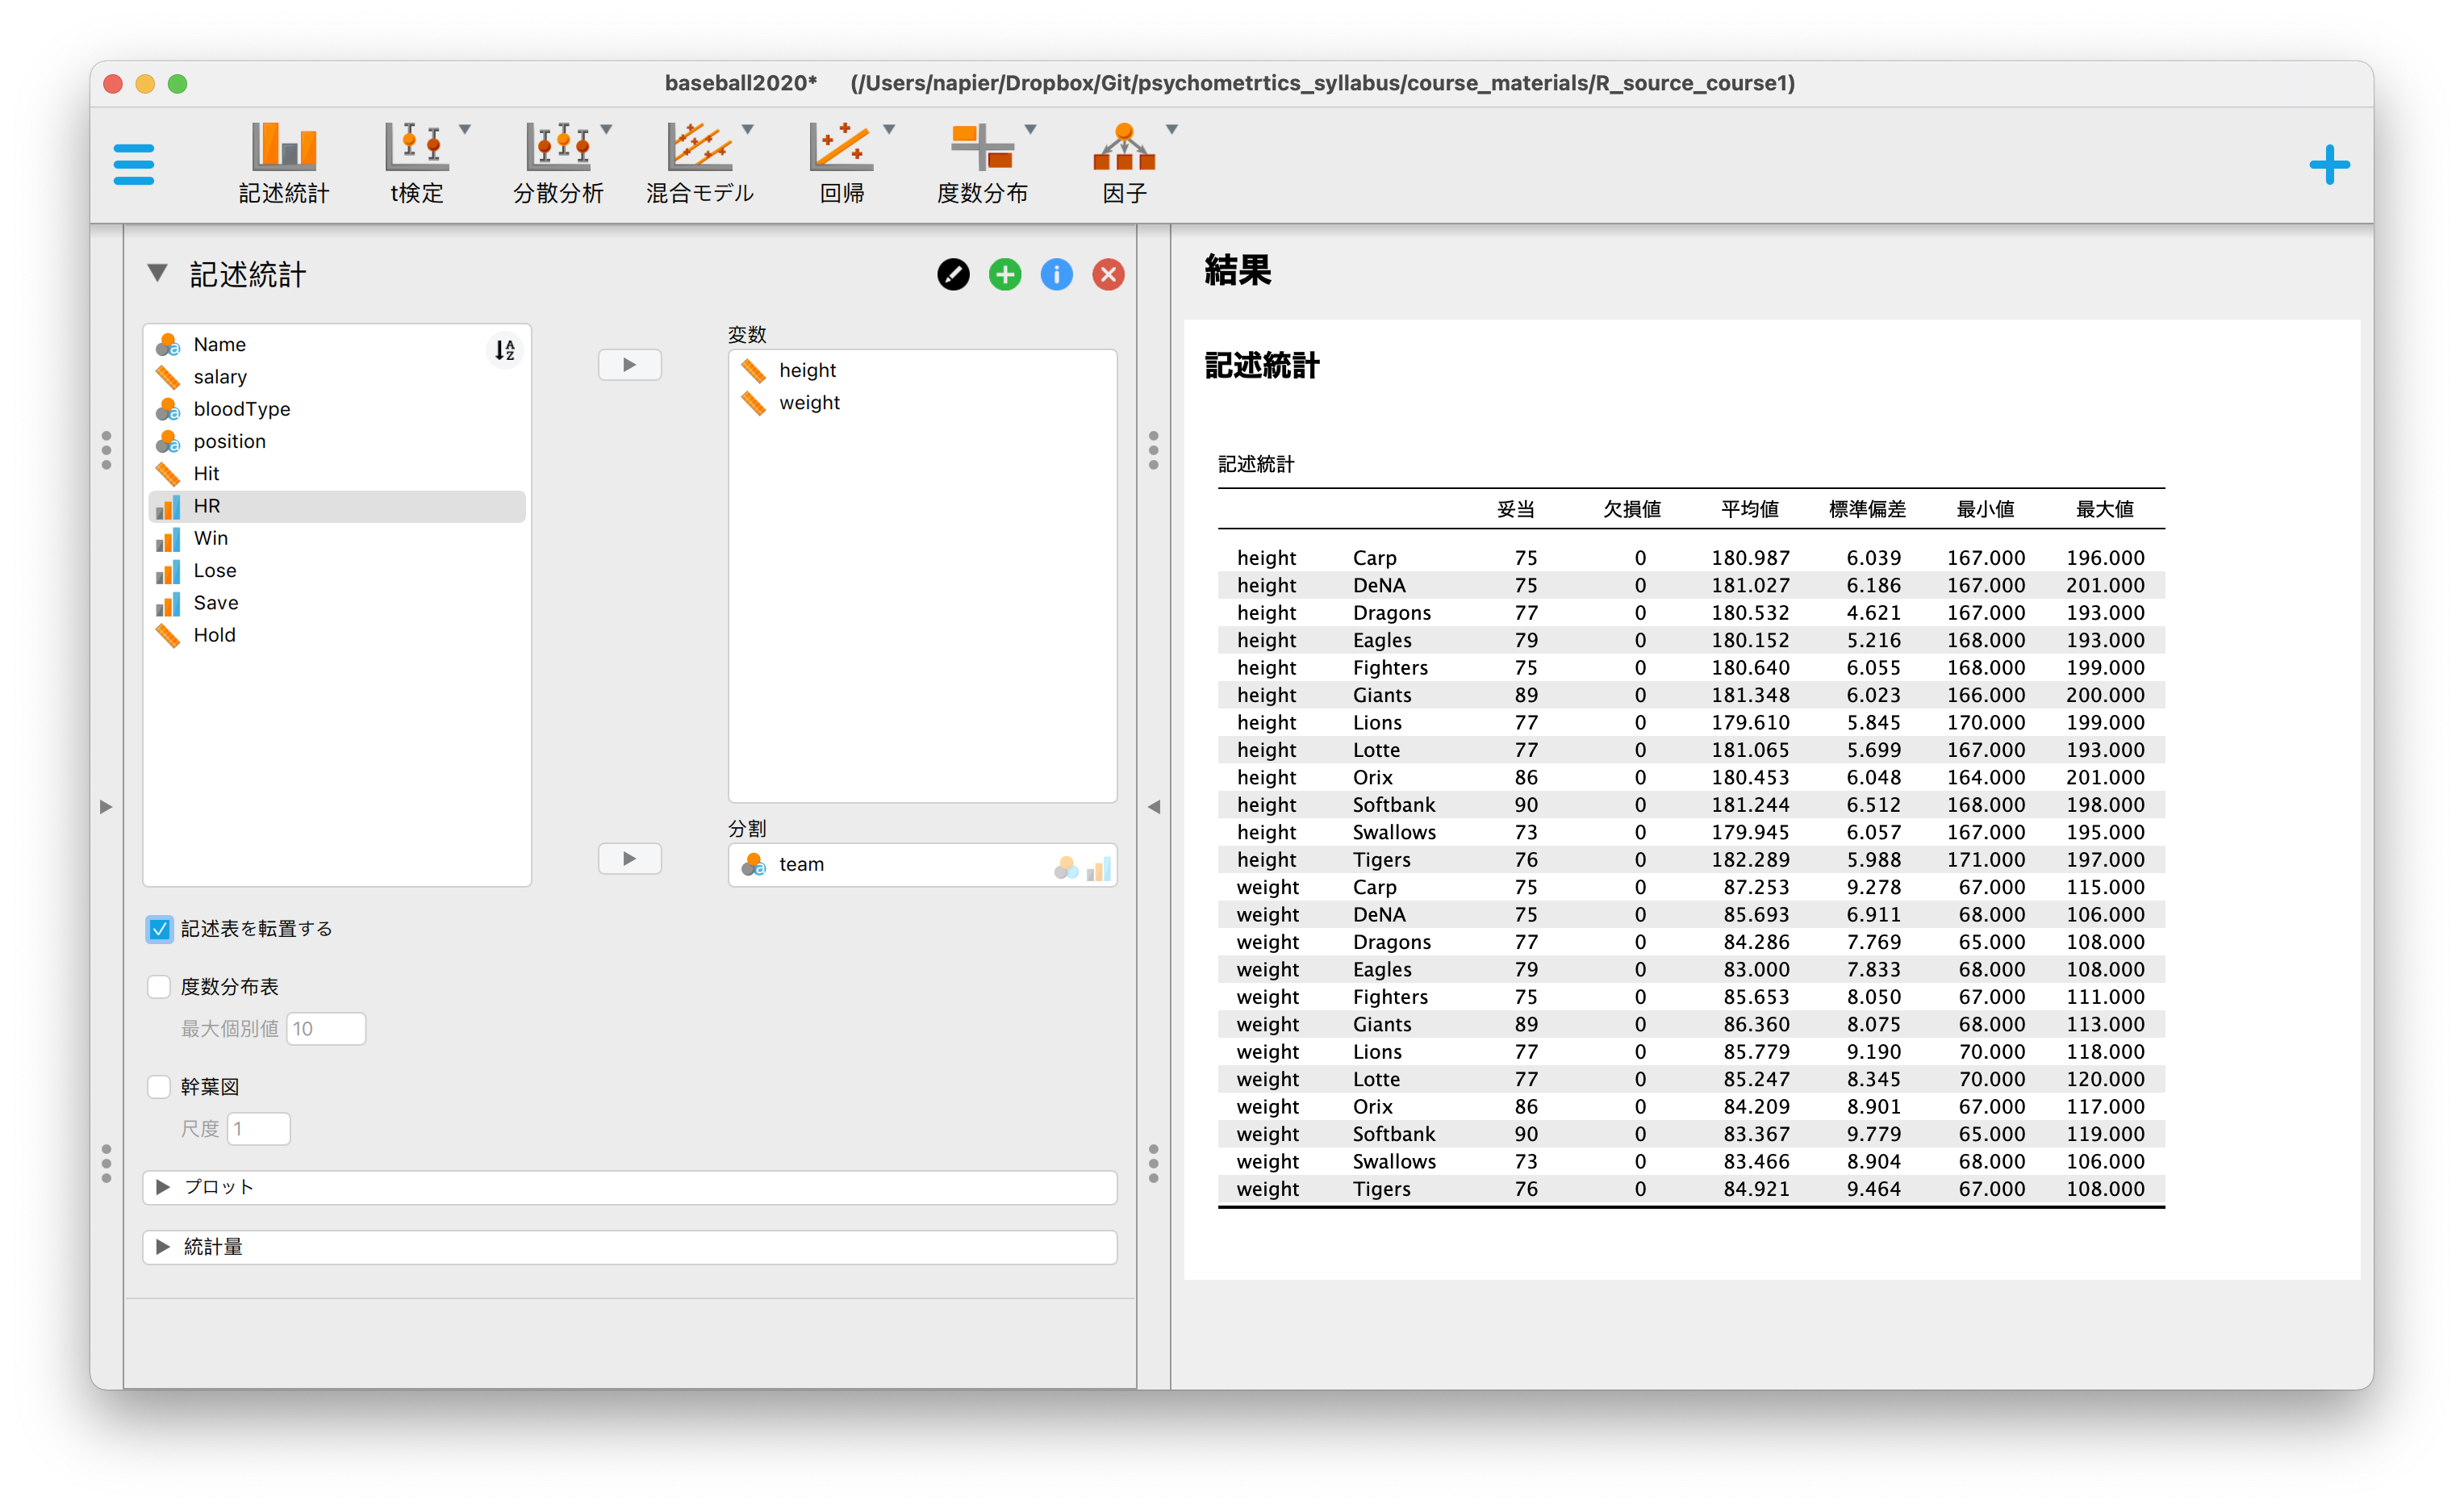
\includegraphics[keepaspectratio,width=0.8\linewidth]{../images/28_JASP/JASP_03.png}
   \caption{Output of descriptive statistics.}
   \label{fig::28_10}
\end{figure}


The descriptive statistics menu has options for "plots" and "statistical measures" that can be specified towards the bottom.
Clicking here will display various options. For example, in plotting, you can choose a color palette for specifying colors, and additional features such as box plots, scatter plots, and regression lines can be selected (see Figure \ref{fig::28_10}).
\begin{figure}[ht]
   \centering
   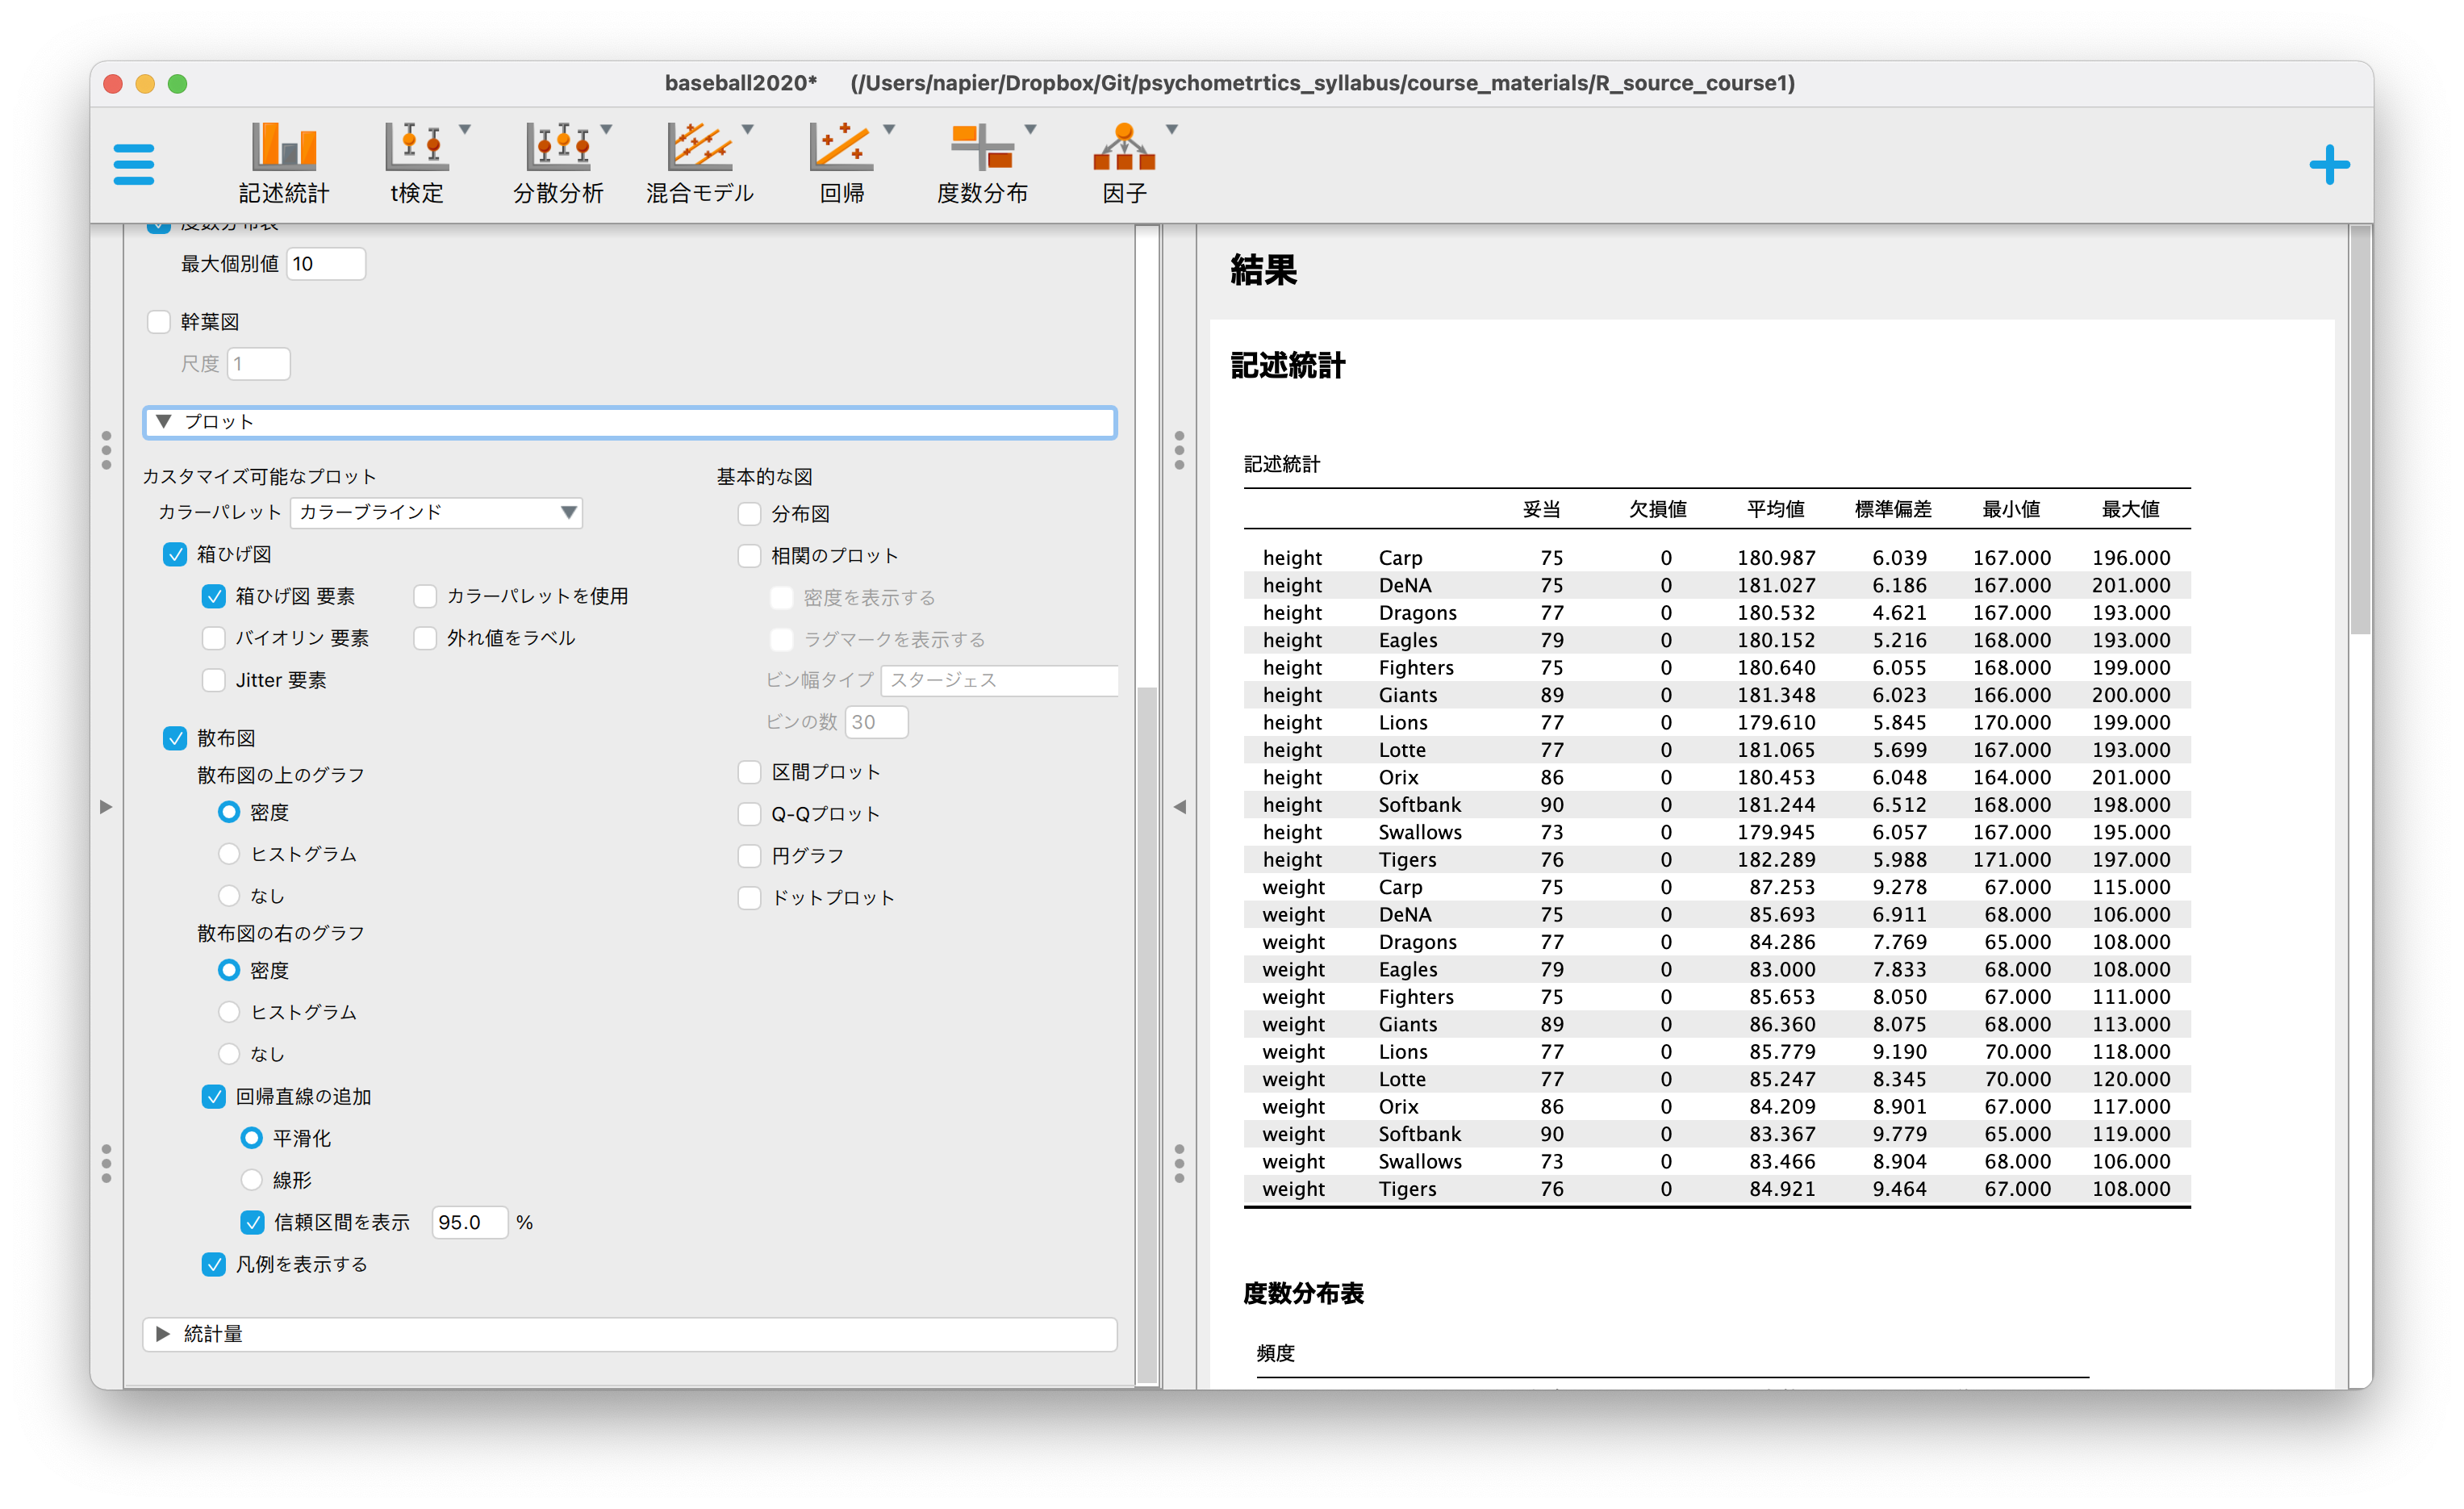
\includegraphics[keepaspectratio,width=0.75\linewidth]{../images/28_JASP/JASP_04.png}
   \caption{Plot options}
   \label{fig::28_11}
\end{figure}


\begin{figure}[ht]
	\centering
	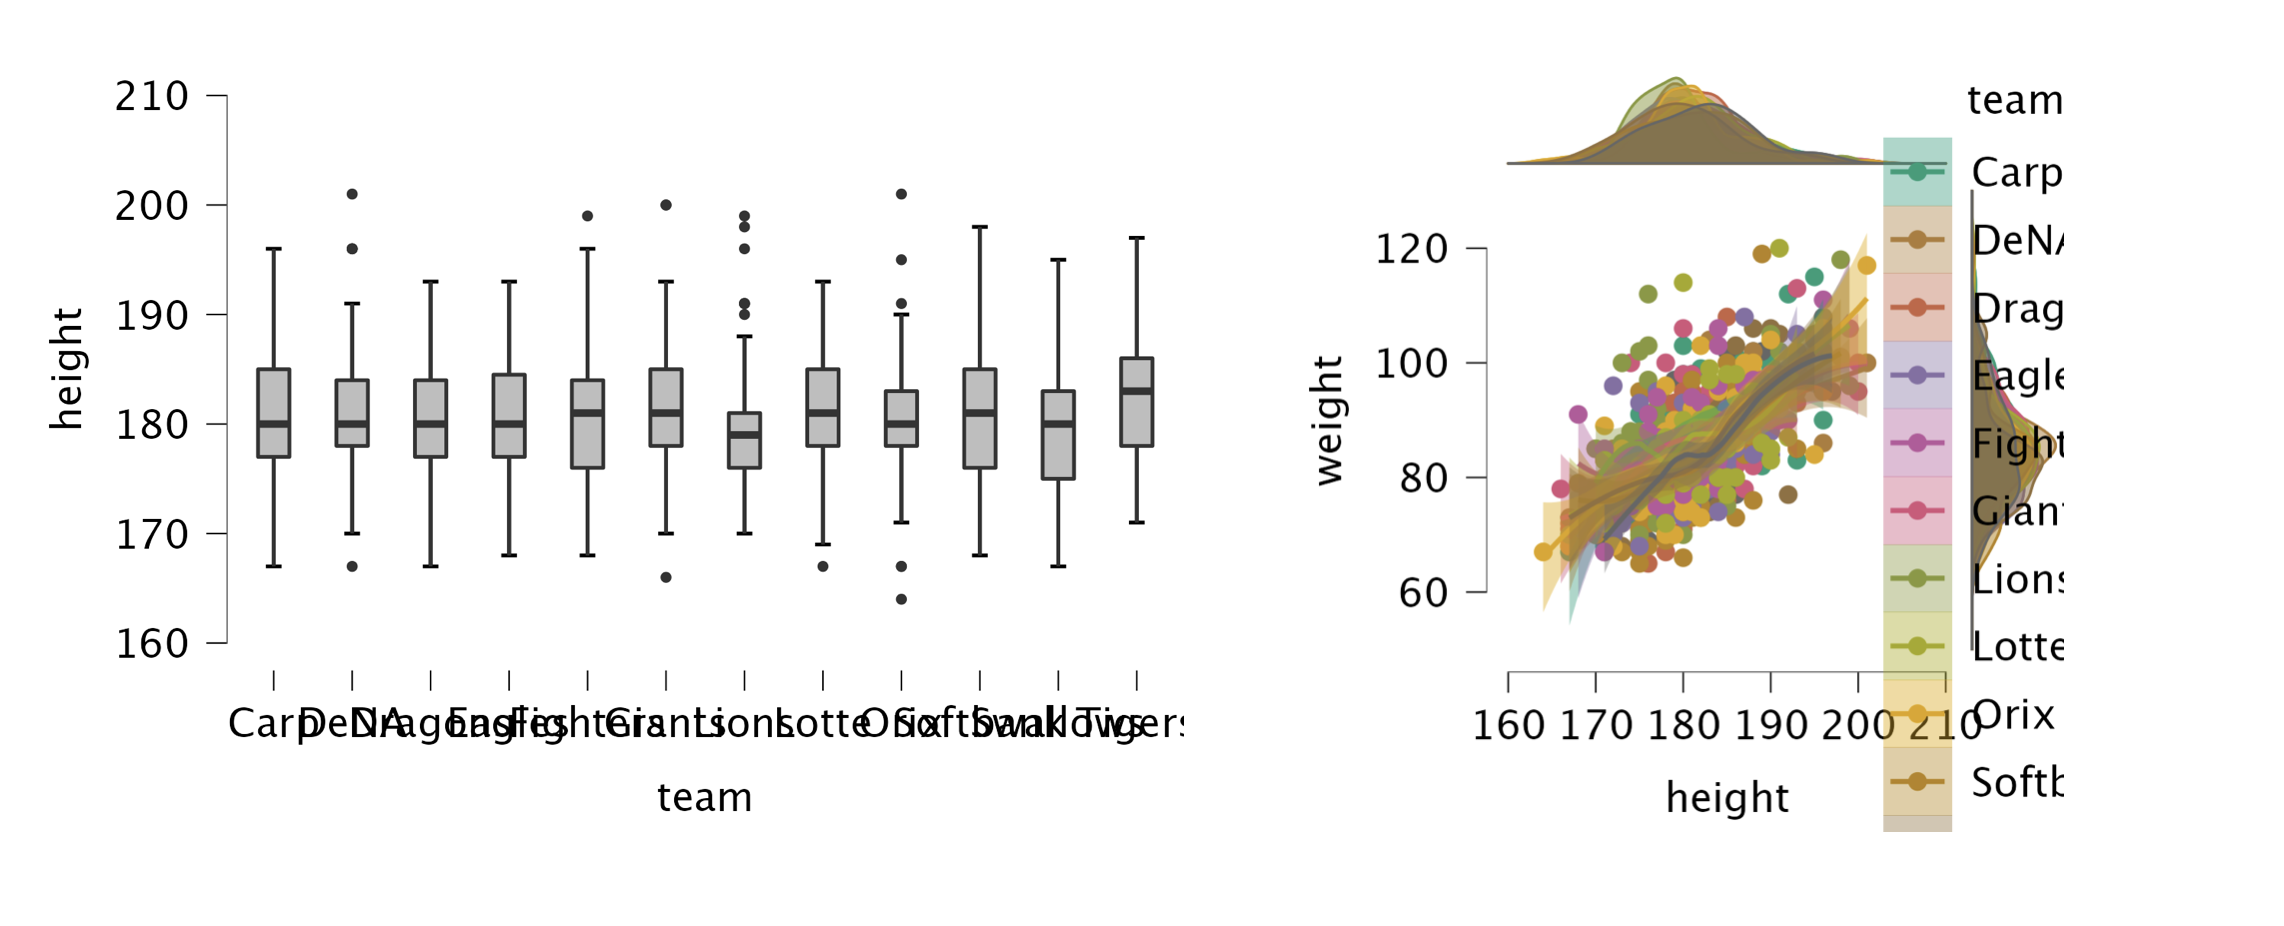
\includegraphics[keepaspectratio,width=0.8\linewidth]{../images/28_JASP/JASP_plot01.png}
	\caption{Box plots and scatter plots}
	\label{fig::28_12}
\end{figure}

Of course, ggplot2 is better suited for fine adjustments of figures, but this should be sufficient to grasp the overall idea\footnote{Although there is an online publication of JASP-compliant text with Japanese translations, there are also descriptions stating that "detailed adjustments are better done with ggplot2." Please see the JASP tutorial website at \url{https://jasp-user-jp.github.io/LSwithJASP/} for more information.}.

These plots can also be copied or saved as image files by clicking the lower triangle beside the figure without modifying the TeX code (Figure \ref{fig::28_13}).
\begin{figure}[ht]
	\centering
	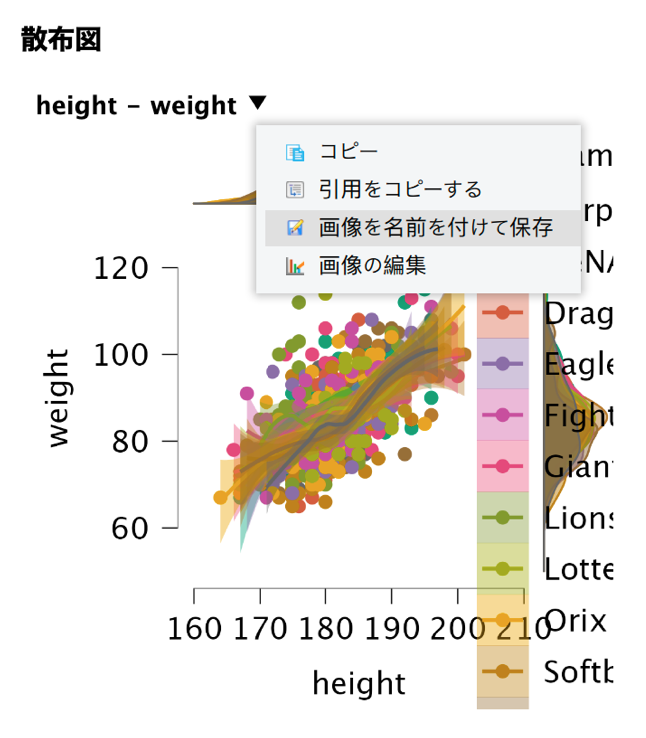
\includegraphics[keepaspectratio, width=0.5\linewidth]{../images/28_JASP/JASP_plot02.png}
	\caption{JASP's figure object can be saved}
	\label{fig::28_13}
\end{figure}

If JASP is capable of adjusting the images without modifying the TeX code, it can be used for creating presentation materials, for example.

\section{Correlation and Regression Analysis with JASP}
As already mentioned, one of the features of JASP is the ability to perform a single analysis using both conventional (based on frequentist probability) and Bayesian (based on subjective probability) methods in parallel. When you click on the menu, you can choose between the traditional and Bayesian approaches (Figure \ref {fig :: 28_14}).
\begin{figure}[ht]
	\centering
	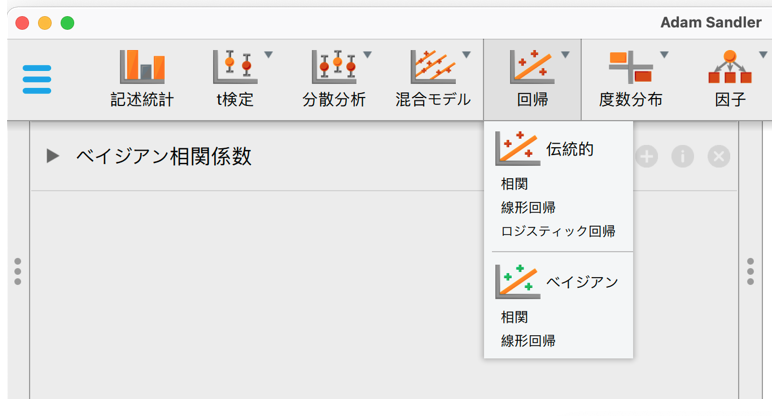
\includegraphics[keepaspectratio,width=0.65\linewidth]{../images/28_JASP/JASP_05.png}
	\caption{Two analyses in one menu}
	\label{fig::28_14}
\end{figure}

Another feature is that there is an abundance of sample data.
Not only can JASP access sample data, but it can also access research data that is publicly available on the web called OSF\footnote{Open Science Framework, an activity that suggests publishing raw data used in research in response to reproducibility issues in psychology, etc. For further information, please refer to \url{https://osf.io/gceur/}.}, and retrieve data from there (Figure \ref{fig::28_15}).
\begin{figure}[ht]
	\centering
	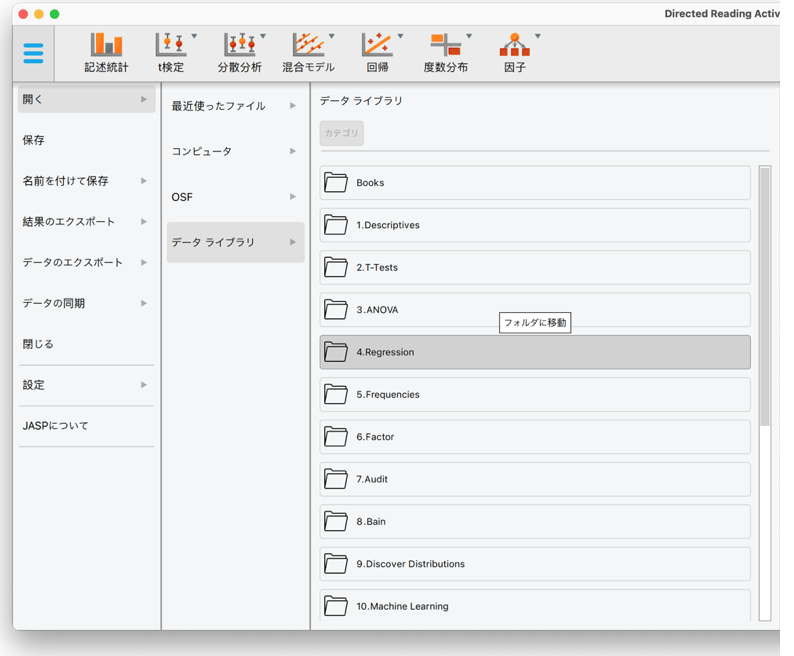
\includegraphics[keepaspectratio,width=0.65\linewidth]{../images/28_JASP/JASP_06.png}
	\caption{There is also an abundance of sample data.}
	\label{fig::28_15}
\end{figure}


Let's select some suitable sample data here and take a look at the correlation coefficient and regression analysis.
I have chosen the data called "Big5". If you go to the data library $\to$ 4.Regression $\to$ Big Five Personality Traits, you can see the data. This is a well-known personality psychology concept that consists of 5 dimensions of personality that are revealed through the results of personality tests. These dimensions are: Openness, Conscientiousness, Extraversion, Agreeableness, and Neuroticism. As this data is related to personality scores, there are likely to be correlations with other variables.

If you simply want a regular correlation coefficient, select Regression from the menu, then select Traditional/Correlation. Just move all the variables to the box on the right and the correlation matrix will be displayed in the results section.
\begin{figure}[ht]
   \centering
   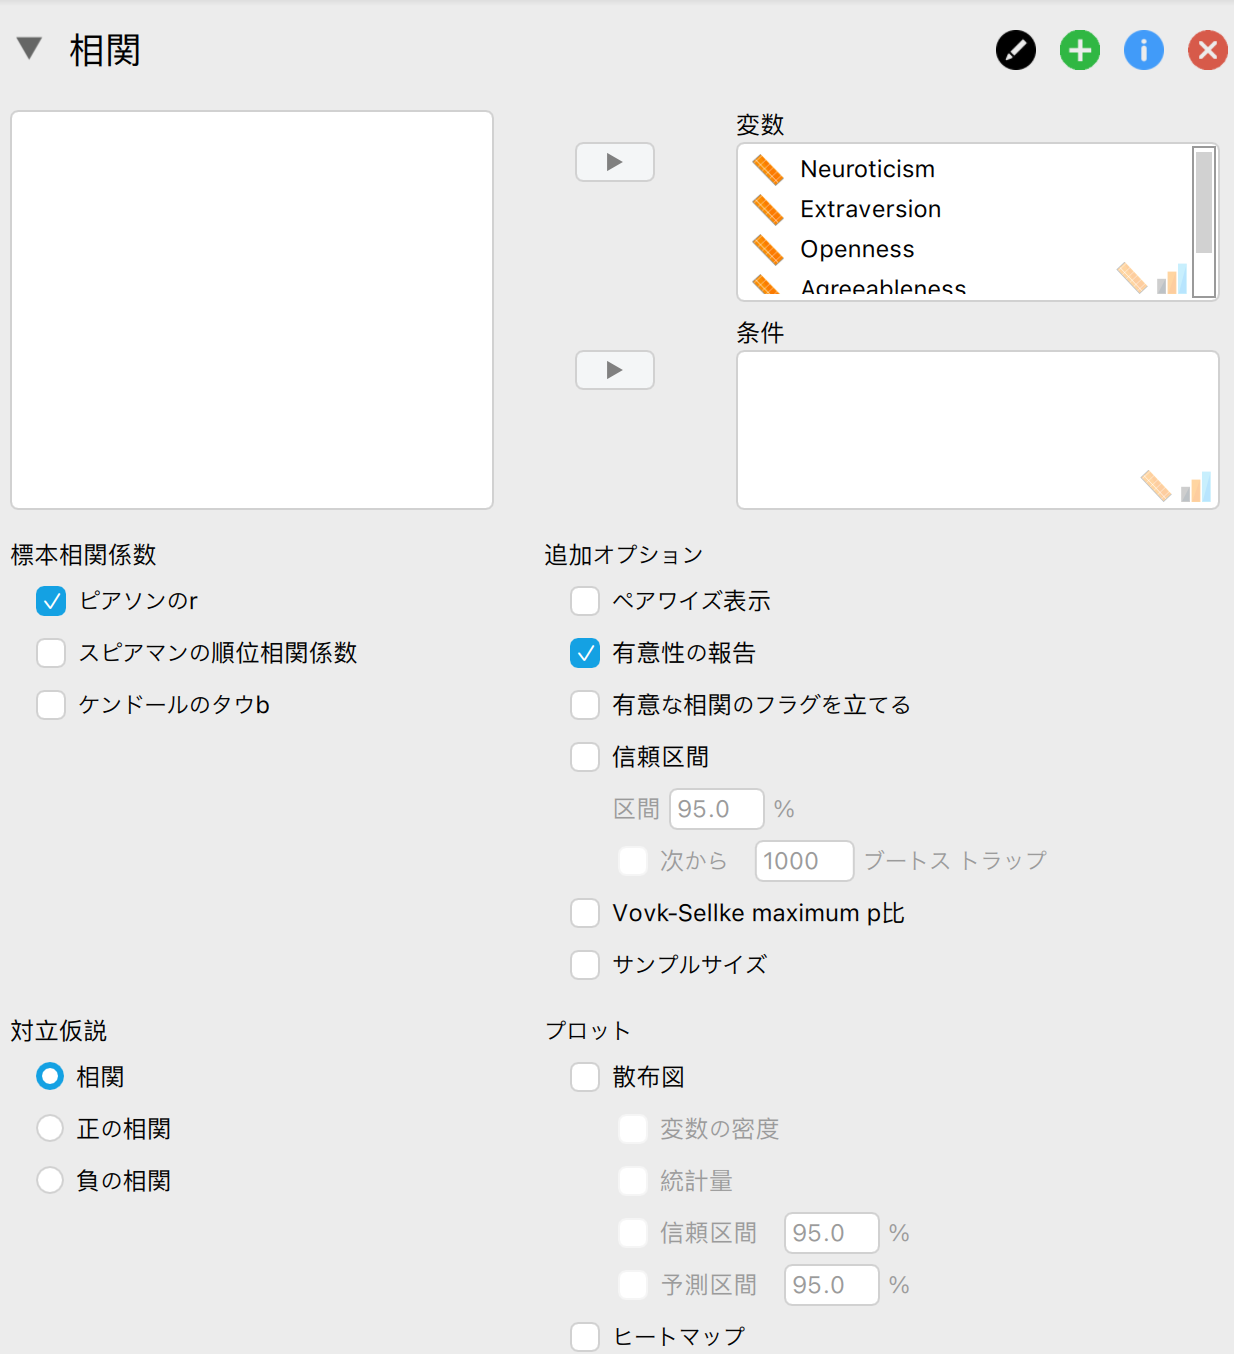
\includegraphics[keepaspectratio,width=0.5\linewidth]{../images/28_JASP/JASP_cor1.png}
   \caption{Traditional correlation analysis}
   \label{fig::28_16}
\end{figure}

The default options have checkboxes for "Pearson's r" and "reporting significance."
The so-called correlation coefficient is formally called the \textbf{Pearson product-moment correlation coefficient}, but in JASP it can also be calculated as Spearman's rank correlation coefficient, which can be applied to data measured on ordinal scales, or as Kendall's tau-b correlation coefficient. The report of significance is accompanied by a checkmark, and the $p$-value is displayed in a table. Please remember that we are comparing the model that assumes a null hypothesis of no correlation between the variables, that is, the population correlation coefficient $\rho$ is zero, and the alternative hypothesis that the population correlation coefficient is non-zero. For example, the correlation coefficient between neuroticism and extraversion is $r=-0.3650$, and the data obtained from this point are somewhat unusual if we assume that the population correlation $\rho=0$ ($p<.001$). By checking the box "Flag significant correlations", asterisks are added to indicate statistically significant results, with more asterisks indicating smaller $p$-values. However, this is a bad habit! A small $p$-value does not necessarily mean a large correlation, and does not provide evidence for the correctness of the hypothesis.

Let's try the same analysis with a Bayesian approach. Simply go to Regression -> Bayesian Correlation in the menu. The selection of variables is also the same procedure.
The additional option for analysis results includes the Bayes factor instead of $p$-values.
The models being compared here are similar to non-Bayesian analyses, where we compare model 0 with a zero population correlation to model 1, which allows for a non-zero population correlation. This comparison is done using the Bayes factor, $BF_{10}$, which represents the ratio of how much the data supports model 1 compared to model 0.
Just now, a statistically significant correlation between neuroticism and extraversion was found, supporting Model 1 by a factor of 6.765e+12, or 6.765 trillion. Bayes factors can sometimes be very large numbers, and can also be influenced greatly by changing the prior distribution, so it may be safe to assume that the factor is not zero.

Let's check the confidence interval instead. The 95\% \underline{confidence interval} is [-0.270, -0.424], which means it is highly unlikely for the correlation coefficient to be larger (closer to 0) than -0.270, probably around 2.5\% chance. Depending on how much we set the \keytermE{ROPE}{Region of Practical Equivalence} to be, we should conclude that it is not at the same level as being uncorrelated.
By the way, the confidence interval using the conventional method is [-0.271, -0.425]. It is almost the same as the Bayesian credible interval. However, in this case, there is a 95% probability that the true correlation coefficient is contained within this interval. In other words, it means "the probability of mistakenly stating that the correlation coefficient exists within this range is 5%."

\section{Comparing Means}
Now, let's compare the average values as a final step.
From the main menu, navigate to Open $\to$ Data Library $\to$ 2.T-Tests$\to$ and select Directed Reading Activities located at the top. It seems to be an experiment plan that examines differences between an experimental group and a control group.
Select t-test for traditional and independent samples from the menu.
Therefore, the only scaling variable "drp" is entered as a dependent variable and "group" is inserted as a grouping variable.
Let's choose both Student's t-test assuming homogeneity of variance and Welch's method, which doesn't assume the process.
The alternative hypothesis assumes that there is a difference between two groups (Group 1 $\neq$ Group 2), and we can choose to check assumptions or effect sizes as appropriate. Please note that the TeX code should not be modified.
\begin{figure}[ht]
   \centering
   
\includegraphics[keepaspectratio,width=0.5\linewidth]{../images/28_JASP/JASP_ttest.png}
   \caption{Traditional t-test}
   \label{fig::28_17}
\end{figure}

As a result, Table \ref{tab:ttest} is shown. In the case of the assumption of equal variances, you can see from the Student's row that $t(42)=-2.267, p=0.029, d=-0.684$ \footnote{The $t$-distribution is named after the pen name "Student" used by William Sealy Gosset, who wrote a paper on it. Unadjusted t-tests for heteroscedasticity are called Student's t-tests. Gosset worked for the Guinness Brewery and was not allowed to publish papers under his real name, hence the pen name.}.

If corrections are necessary, refer to Welch. Then, it is found that $t(37.855)=-2.311$, $p=0.026$, and $d=-0.691$.
%----- Requires booktabs package -----%


\begin{table}[ht]
	\centering
	\caption{Independent sample t-test}
	\label{tab:ttest}
	{
		\begin{tabular}{lrrrrr}
			\toprule
			$ $ & Test    & Statistic & df       & p-value & Cohen's d \\
			\cmidrule[0.4pt]{1-6}
			drp & Student & $-2.267$  & $42.000$ & $0.029$ & $-0.684$  \\
			$ $ & Welch   & $-2.311$  & $37.855$ & $0.026$ & $-0.691$  \\
			\bottomrule
		\end{tabular}
	}
\end{table}


When should we refer to the Student row, and when should we refer to the Welch row? In general, it is best to refer to the Welch row which has looser assumptions, but whether or not we can assume equal variances can be determined through checking the "assumption."
There is a Shapiro-Wilk test (Table \ref{tab:Shapiro-Wilk}) used to test whether the data follows a normal distribution, which is a fundamental assumption to begin with when making assumptions. Next, there is a Levene test (Table \ref{tab:Levene}) used to test whether the variances can be considered the same.

Please note that these tests have a null hypothesis of "following a normal distribution" and "having equal variance", and an alternative hypothesis of "not following" and "not having equal variance", respectively. That is, when the analysis results are statistically significant, it means that "they do not follow" and "they do not have equal variance". If the Shapiro-Wilk test is statistically significant, you should not perform a t-test in the first place. If the Levene's test is statistically significant, it means that the assumption of equal variance has been violated, so you should look at Welch's test instead.
%----- Requires booktabs package -----%

\begin{table}[ht]
   \centering
   \caption{Normality test (Shapiro-Wilk)}
   \label{tab:Shapiro-Wilk}
   {
      \begin{tabular}{lrrr}
         \toprule
             &         & W       & p       \\
         \cmidrule[0.4pt]{1-4}
         drp & Control & $0.972$ & $0.732$ \\
         $ $ & Treat   & $0.966$ & $0.652$ \\
         \bottomrule
         % \addlinespace[1ex]
         % \multicolumn{4}{p{0.5\linewidth}}{\textit{Note} significant results suggest deviation from normality.} \\
      \end{tabular}
   }
\end{table}

%----- Requires booktabs package -----%
Fortunately, in this case, the result of the Levine's test was not significant with $p=0.132$, so we can proceed with the Student's t-test.
\begin{table}[ht]
	\centering
	\caption{Levene's test for homogeneity of variances}
	\label{tab:levene}
	{
		\begin{tabular}{lrrr}
			\toprule
			    & F       & df  & p       \\
			\cmidrule[0.4pt]{1-4}
			drp & $2.362$ & $1$ & $0.132$ \\
			\bottomrule
		\end{tabular}
	}
\end{table}

It's a bit cumbersome, isn't it? In the hypothesis testing phase, we support the null hypothesis, but in the actual testing phase, we support the alternative hypothesis. It makes me want to say, "I thought we weren't supposed to actively support the null hypothesis!" And because we're repeating the testing process, the level of significance may no longer be 5%.

No such anxiety is needed in the case of Bayesian statistics. Let's proceed with Bayesian analysis right away.
Next, select t-test for Bayesian independent samples from the menu.
The selection process for dependent variables and grouping variables is the same.

The result was shown as Table \ref{tab:bayesianTtest}. Since $BF_{10}=2.217$, the alternative hypothesis (Model 1) that there is a difference is supported about 2.2 times more than the null hypothesis (Model 0) which assumes no difference. In other words, the alternative hypothesis is somewhat more favorable. However, it is premature to conclude that "there is a difference" since a general rule of thumb for BF is that it should be greater than 3.
%----- Requires booktabs package -----%

\begin{table}[ht]
   \centering
   \caption{Bayesian independent sample t-test}
   \label{tab:bayesianTtest}
   {
      \begin{tabular}{lrr}
         \toprule
             & BF$_{1}$$_{0}$ (Bayes Factor for alternative hypothesis against null hypothesis) & Error \% \\
            \cmidrule[0.4pt]{1-3}
         drp & $2.217$        & $0.002$   \\
         \bottomrule
      \end{tabular}
   }
\end{table}

Looking at descriptive statistical plots, this becomes clear (see Figure \ref{fig::28_18}).
\begin{figure}[ht]

	\centering
	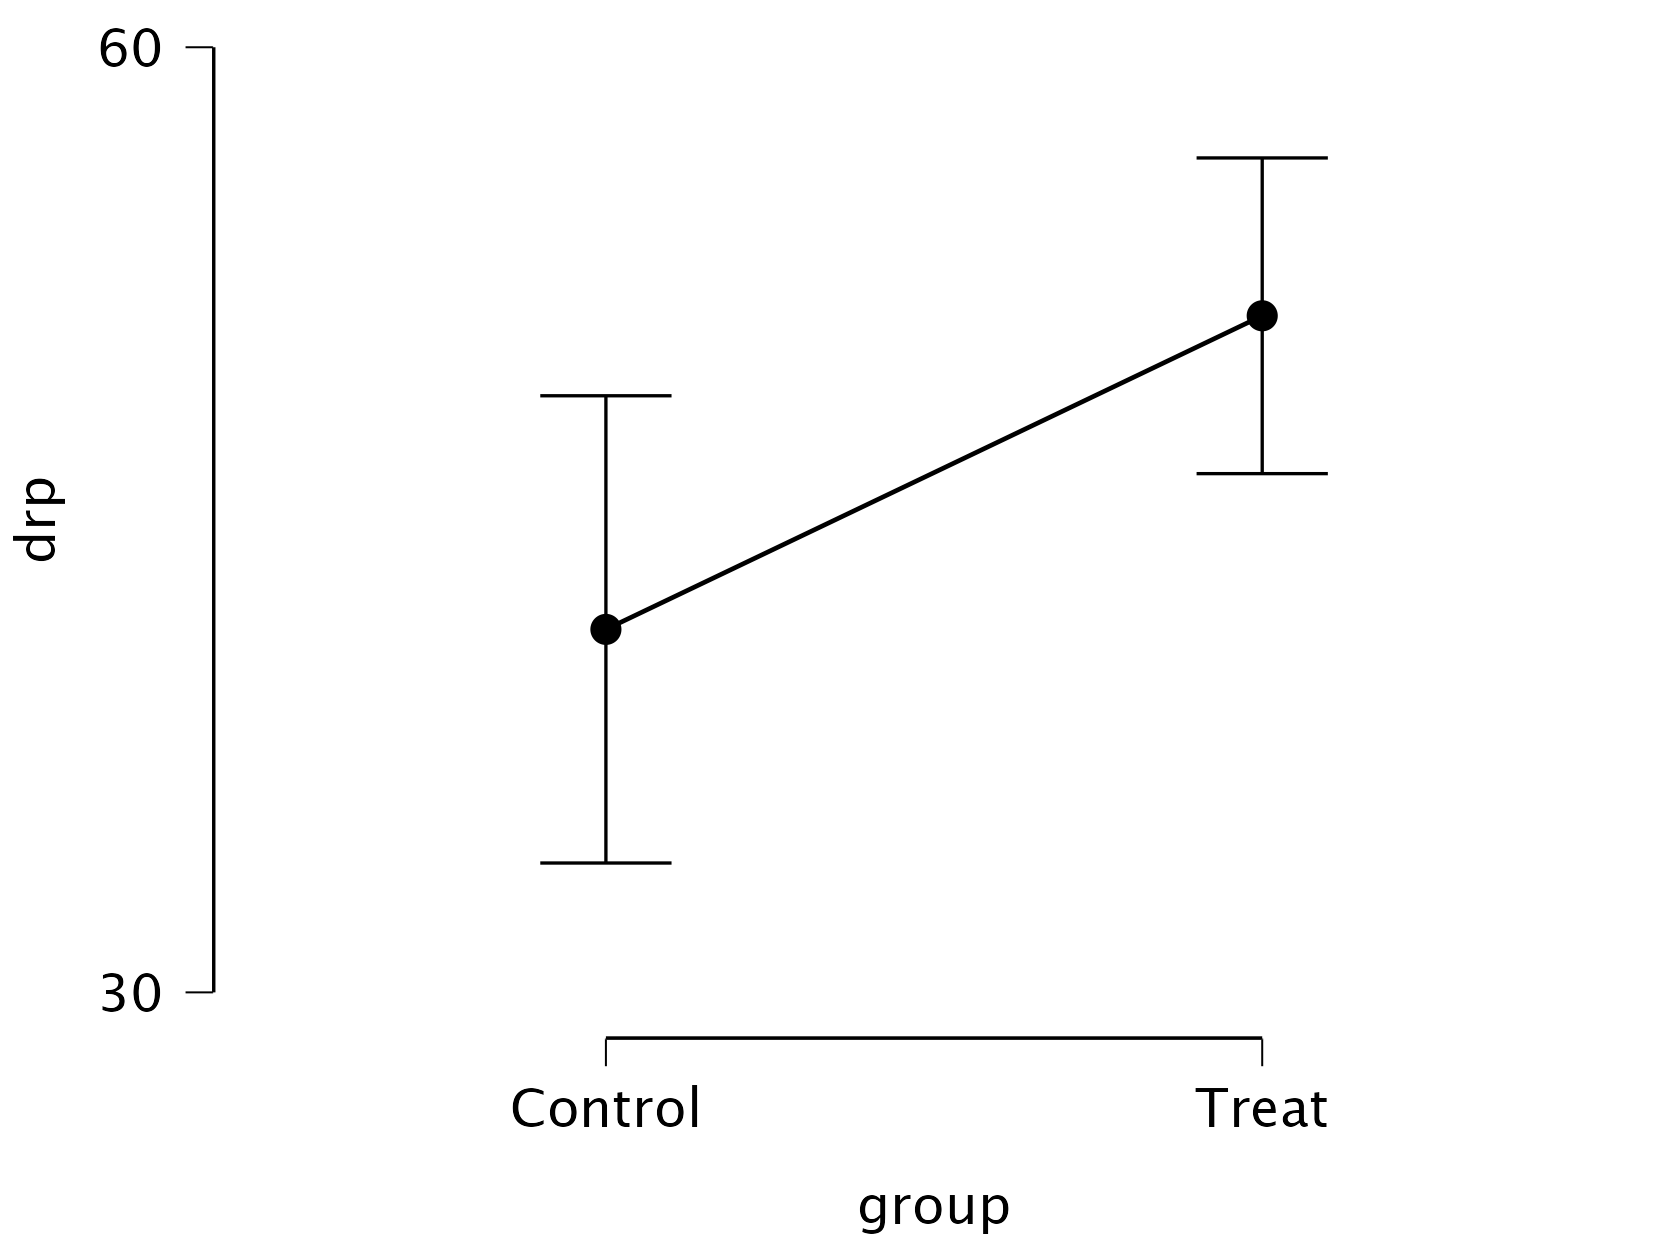
\includegraphics[keepaspectratio,width=0.5\linewidth]{../images/28_JASP/JASP_ttestPlot.png}

	\caption{Mean values and confidence intervals of two groups}

	\label{fig::28_18}

\end{figure}

When looking at this, it seems that the 95% confidence intervals for the experimental and control groups overlap quite a bit. When there is overlap, it's best to hold off on hasty judgments, regardless of the size of the ROPE, and wait to consider the data (evidence) further before making any decisions.

Let's take a look at the output of "prior distribution" and "posterior distribution" (Figure \ref{fig::28_19}), without modifying the TeX code.
\begin{figure}[ht]
   \centering
   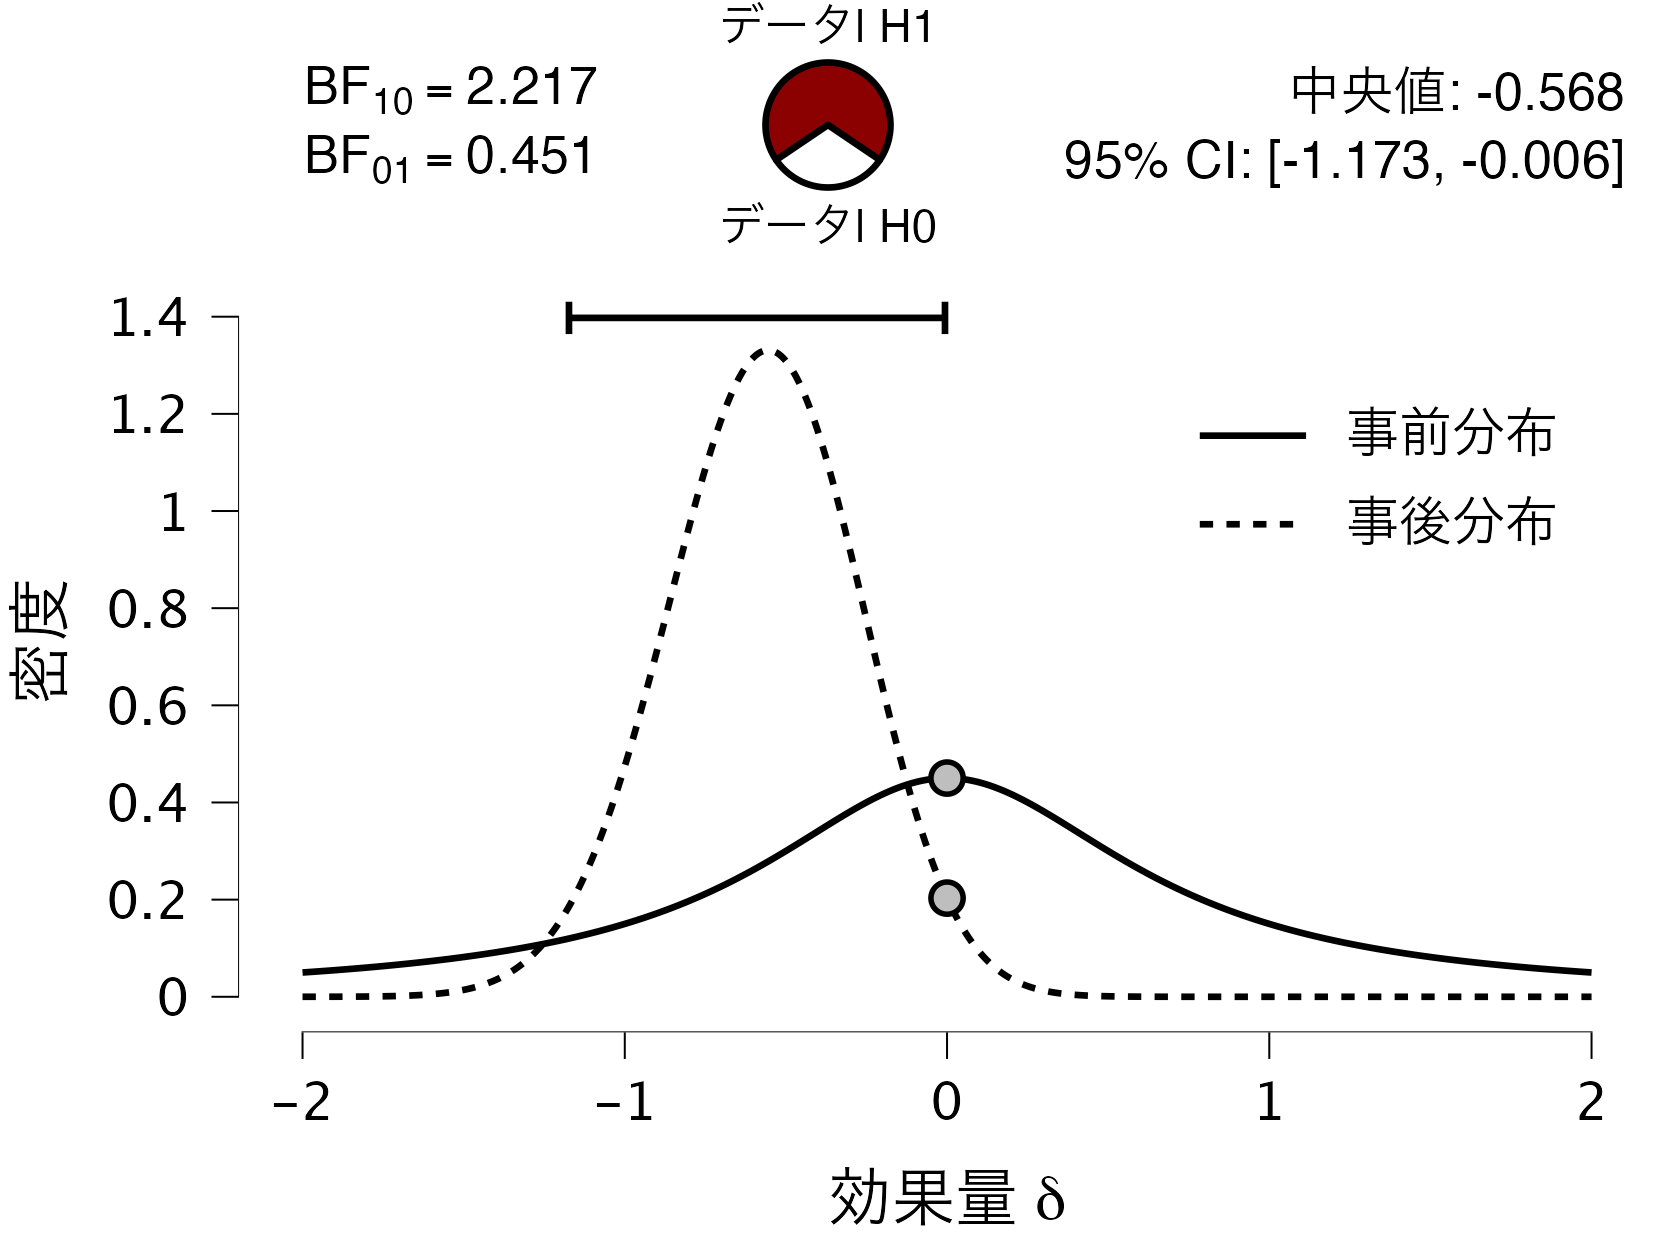
\includegraphics[keepaspectratio,width=0.8\linewidth]{../images/28_JASP/JASP_ttestBF.png}
   \caption{Prior and posterior distributions}
   \label{fig::28_19}
\end{figure}


This shows the prior and posterior distributions of the estimated value $\delta$ of the effect size $d$. The effect size represents the standardized difference in mean values, and in the prior distribution, a Cauchy distribution centered around 0 is assumed. In other words, subjectively, before conducting the test, there is a faint belief that "maybe there's no difference". When we overlay the posterior distribution calculated from the data (i.e. the likelihood and prior probability), we can see that the density at $\delta=0$ is lower than that of the prior distribution.
It is known that the density ratio at a specific point of the prior distribution and the posterior distribution is equal to the Bayes factor, and calculating the Bayes factor using this method is called the Savage-Dickey method\citep{Lee201709}. Calculating the Bayes factor requires integrating the marginal likelihood, which can be difficult, but if there is a relationship between a hypothesis for a point, such as the null hypothesis, and a competing hypothesis that includes it, then the density ratio of the prior and posterior distributions can be used.

Anyway, looking at this, it has only dropped a little. Also, the confidence interval for $\delta$ is [-1.173, -0.006]. The upper limit is almost zero. Zero means there is no difference, so it may be a bit tough to claim that there is a difference with this data.

Here is a note. Some people may think, after seeing the results of both the conventional method and the \keytermE{Bayesian method}{ベイズ法}, "Hmm, if the conventional method shows a significant difference and the Bayesian method doesn't show it as strongly, why not just report the conventional method and hide the fact that there may not be a significant difference?" However, this attitude of "let's hide something that might be bad for me" lacks scientific integrity. In this case, both the results support the alternative hypothesis, but if the difference is more subtle, the results of the conventional method and the Bayesian method might differ. Whether there is a difference or not, it is important to consider "what this data is really telling us" by carefully thinking about both results. It is more important to strive for a correct understanding of the phenomenon, rather than selectively using only favorable results or making shortsighted judgments about whether there is a difference or not. Therefore, it is important to report all of the confidence intervals, credible intervals, $p$ values, effect sizes, Bayesian factors, and everything else, and work on truly understanding the phenomenon.


Anyway, by using a software called JASP, it became clear that both methods can be easily compared. In the future, we can expect to see more research examples reporting analysis results in the form of a combination of t-test and BF.
Please try various data analysis through JASP, too.
\end{document}
